\documentclass[a4paper, 12pt, twoside]{report}

% This can be used if you want to increase the spacing between lines to 1.5x
%\linespread{1.5}

%General packages

% Uncomment the following line for preparing the final hardcopy (and comment out the next one)
\usepackage[a4paper,left=40mm,right=20mm,top=30mm,bottom=20mm]{geometry}
% Use this for your draft (easier to read). Don't forget to manually check
% everything when you switch to final hardcopy geometry (see above)
%\usepackage[a4paper,left=20mm,right=20mm,top=30mm,bottom=20mm]{geometry}
\usepackage[spanish]{babel}
% \usepackage[utf8]{inputenc}
\usepackage{graphicx}
\usepackage{gensymb}
\usepackage{textcomp}
\usepackage{amsfonts}
\usepackage{appendix}
\usepackage{listings}
\usepackage{float}
%\lstset{breaklines=true}
%\DeclareGraphicsExtensions{.pdf,.jpeg,.png}
\usepackage{amsmath}
\usepackage{amssymb}
\usepackage{algpseudocode}
\usepackage{algorithm}
%\usepackage{array}
\usepackage{subfig}
%\usepackage{captcont}
\usepackage{booktabs}
\usepackage[hyphens]{url}
\usepackage{multirow}
\usepackage{parskip}
%\usepackage{cite}
\usepackage[table]{xcolor}
\usepackage{hyperref}
\usepackage{amsfonts}
\usepackage{amsthm}
\usepackage{mathrsfs}
\usepackage{quiver}
\usepackage{enumitem}
\usepackage{placeins}
\newtheorem*{theorem*}{Theorem}
\newtheorem{theorem}{Theorem}[section]
\newtheorem{proposition}{Proposition}[section]
\newtheorem{corollary}{Corollary}[section]
\newtheorem{lemma}{Lemma}[section]
\newtheorem{conjecture}{Conjecture}[section]

\theoremstyle{definition}
\newtheorem{definition}{Definition}[section]
\newtheorem{example}{Example}[section]

\theoremstyle{remark}
\newtheorem*{rem}{Remark}

\newcommand{\mathdefault}[1][]{}

\newcommand\xqed[1]{%
  \leavevmode\unskip\penalty9999 \hbox{}\nobreak\hfill
  \quad\hbox{#1}}
\newcommand\tqed{\xqed{$\triangle$}}
%\newsavebox{\imagebox}

%Formatting for headers and footers
\usepackage{fancyhdr}
\pagestyle{fancy}
\fancyhead{}
%\fancyhead[RO,LE]{Monolithic Nanocomposite Detector for LaBrAT-PET}
\renewcommand{\headrulewidth}{0pt}
\fancyfoot{}
\fancyfoot[LE,RO]{\thepage}
%\fancyfoot[LO,RE]{Student Name}

%Bibliography settings
\usepackage[backend=biber,sorting=none,style=ieee]{biblatex}
\addbibresource{library.bib}

%Link to graphics folder
\graphicspath{{figures/}}

% Set your thesis title and author details here
\title{La Dinámica de Glóbulos Rojos en Medicina: Un acercamiento con Modelos Matemáticos.}
\author{Miguel Sandoval Cardozo}
\date{\today}

\allowdisplaybreaks

\begin{document}

\begin{titlepage}
\begin{center}
%\vspace*{1cm}

\Huge
\makeatletter
\textbf{\@title}

\Large

\vspace{3.cm}

by \textbf{\@author{}}

\vfill
\large
Thesis submitted in fulfilment of the requirements for the degree of\\
\textit{Bachelor of Science}\\
under the supervision of Tristram Bogart\\
\vfill
\large
Department of Mathematics\\
Faculty of Science\\
Universidad de los Andes\\

\today
\makeatother

\end{center}
\end{titlepage}


% \chapter*{Certificate of Authorship / Originality}

\makeatletter

I, \@author{}, declare that this thesis is submitted in fulfilment of the requirements for the award of Doctor of Philosophy, in the School of Electrical and Data Engineering at the University of Technology Sydney.
\makeatother

\vspace{6pt}

\noindent This thesis is wholly my own work unless otherwise referenced or acknowledged. In addition, I certify that all information sources and literature used are indicated in the thesis. This document has not been submitted for qualifications at any other academic institution.

% If applicable, the above statement must be replaced with the collaborative doctoral degree statement (see below).

% If applicable, the Indigenous Cultural and Intellectual Property (ICIP) statement must be added (see below).

\vspace{6pt}

\noindent This research is supported by the Australian Government Research Training Program.

% If you have a top-up or other scholarship, please modify this.

\vspace{1cm}

\begin{tabular}{m{3cm}m{7cm}}
Signature: &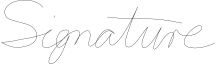
\includegraphics[width=6cm]{example_signature}\\

Date:	&\today\\
\end{tabular}
\vspace{6pt}

\makeatletter

% Can also use a copyright statement as below
%\hfill $\copyright$ Copyright \today{} \@author{}

\makeatother


\pagenumbering{roman}

\chapter*{Resumen}

El modelo discreto que intenta simular el proceso de vida de los glóbulos rojos propuesto por Eldestein en \cite{edelstein1988mathematical} es:

$$R(n+1)=(1-f)R(n)+M(n),$$
$$M(n+1)=\gamma \cdot f\cdot R(n),$$

en donde $R(n)$ representa la cantidad de glóbulos rojos en el día $n$ y $M(n)$ los glóbulos rojos producidos por la médula ósea. El parámetro $0\leq f \leq 1$ representa la fracción de glóbulos rojos filtrados por el bazo diariamente y $\gamma \geq 0$ representa la cantidad de RBC's producidos por la médula ósea por cada uno eliminado por el bazo. 

En el proyecto se hace un análisis matemático de este modelo base y se hacen tres simulaciones computacionales cambiando el valor de $\gamma$ (tomándolo mayor, menor o igual a 1). Cada simulación es analizada según las observaciones hechas desde el punto de vista matemático. 

Posteriormente se presentan tres variaciones del modelo siguiendo tres principales complicaciones médicas: una hemorragia leve (pérdida de sangre del $2\%$), una hemorragia grave (pérdida de sangre del $14\%$) y anemia renal (deficiencia de eritropoyetina). Para cada uno de los casos se presenta su tratamiento médico, su correspondiente simulación computacional y el análisis de esta. 

Para concluir se presentan nuevas variables a tener en cuenta a la hora de proponer el modelo y algunos cambios que se podrían hacer para modificar los resultados obtenidos. También se propone un trabajo a futuro para incluir al modelo la movilización de células madre para pacientes con cáncer.



\chapter*{Dedicatoria}
\textit{Para Ramiro, mi héroe.}



\chapter*{Agradecimientos}
El primer agradecimiento es para el profesor José Ricardo Arteaga, por introducirme al mundo de los modelos matemáticos, por su fantástica labor como asesor y como consejero de vida. A Jorge Duitama quiero agradecerle por brindarme herramientas computacionales que fueron muy importantes para el trabajo y por todo el apoyo que me ha brindado. Al doctor Óscar Peña MD, hematólogo enfocado en trasplante de médula ósea, por sus valiosas lecciones médicas que fueron clave para entender el problema. Adicionalmente quiero agradecer a los miembros de los departamentos de matemáticas y literatura de la Universidad de los Andes, pues todas sus enseñanzas han sido fundamentales para mi formación profesional. Finalmente quiero agradecer a mi familia y a mis amigos, sin quienes nunca hubiera llegado tan lejos.   




{
\makeatletter
\vspace{1cm}
\raggedleft
\@author{}\\
\today{}\\
Bogotá, Colombia\\
\raggedright
\makeatother
}


\tableofcontents
%\listoffigures
%\listoftables

\pagenumbering{arabic}

% Add additional chapters as required
\chapter{Introducción}\label{chap:intro}

\section{Presentación del tema y su importancia}

El proyecto de investigación a continuación presentará una aproximación teórica para tratar de comprender un problema médico utilizando herramientas matemáticas. La principal herramienta utilizada son los modelos matemáticos, otra herramienta utilizada es la simulación computacional de cada modelo propuesto. 

\textbf{Presentación del problema:} Los glóbulos rojos pertenecen al aparato circulatorio del cuerpo humano, siendo las células que componen mayoritariamente la sangre. Entre sus diferentes funciones se encuentra el transporte de oxígeno desde los pulmones al resto de órganos del cuerpo para garantizar su funcionamiento. Es por este motivo que medir la cantidad de glóbulos rojos en la sangre de una persona permite prevenir complicaciones médicas.

Los hemogramas son procedimientos médicos para hacer un análisis completo de la sangre de una persona. Siguiendo el artículo de Celkan en \cite{celkan2020does}, para hacer un hemograma se extrae una pequeña cantidad de sangre que se envía a un laboratorio y se analiza. Así, poder determinar la cantidad de glóbulos rojos en una persona en todo momento es una tarea imposible, pues se necesitaría una cantidad infinita de sangre y equipo que pudiera hacer las mediciones inmediatamente. Es por esto que el problema de la medición de glóbulos rojos es muy importante en el mundo médico, una de las aproximaciones al problema es mediante los modelos matemáticos.

\textbf{Herramientas:} Un modelo matemático es un sistema de ecuaciones discretas (es decir que su medición es cada cierto intervalo de tiempo) o continuas que intenta reflejar ciertos comportamientos del mundo real en ámbitos como la economía o la medicina. Para acercarse al problema de las dinámicas de los glóbulos rojos (RBC's), Leah Edelstein-Keshet en \cite{edelstein2005} propuso el siguiente modelo que intenta reflejar la vida de los glóbulos rojos dentro del cuerpo humano:

$$R(n+1)=(1-f)R(n)+M(n),$$
$$M(n+1)=\gamma \cdot f\cdot R(n),$$

en donde $R(n)$ representa la cantidad de glóbulos rojos en el día $n$ y $M(n)$ los glóbulos rojos producidos por la médula ósea. El parámetro $0\leq f \leq 1$ representa la fracción de glóbulos rojos filtrados por el bazo diariamente y $\gamma \geq 0$ representa la cantidad de RBC's producidos por la médula ósea por cada uno eliminado por el bazo. 

Este modelo, como se expondrá en la sección \ref{sec:modelo:presentacion}, es válido desde un punto de vista médico, por lo que se puede intentar adoptar para resolver el problema propuesto. 

\section{Objetivos del trabajo}

El objetivo principal del proyecto es determinar si el modelo de Edelstein-Keshet es correcto desde un punto de vista médico y matemático, determinando sus equilibrios y haciendo simulaciones computacionales al variar valores del parámetro $\gamma$, la cantidad de glóbulos rojos producidos por cada uno perdido.

El modelo base, al estar basado en un paciente totalmente sano, no tiene en consideración posibles complicaciones médicas que pueda sufrir un paciente, por lo que el siguiente objetivo del trabajo es incluir en el modelo ciertas enfermedades como hemorragias o anemia y sus respectivos tratamientos médicos, todo esto después de haber realizado una investigación médica. Para el caso de un paciente con anemia, esta debe ser tratada con inyecciones del fármaco llamado eritropoyetina, de esta manera, otro de los objetivos es encontrar una dosis de eritropoyetina que satisfaga los resultados esperados. Para el caso de las hemorragias, se buscarán evidenciar los beneficios de una transfusión sanguínea.

\section{Estructura del documento}

El documento está dividido en cuatro capítulos (excluyendo el presente) que muestran el desarrollo y cumplimiento de los objetivos previamente mencionados:

\begin{itemize}
    \item El capítulo \ref{chap:RBC} presenta la investigación médica realizada sobre los glóbulos rojos, sus dinámicas dentro del cuerpo y el estudio de las hemorragias y la anemia y sus respectivos tratamientos;
    \item dado este trasfondo médico, el capítulo \ref{chap:modelo} presenta el análisis matemático del modelo base, su justificación desde el punto de vista médico y tres simulaciones computacionales con su respectivo análisis;
    \item habiendo ya analizado el modelo base, el capítulo \ref{chap:variaciones} presenta las variaciones del modelo para incluir en este las enfermedades presentadas junto son sus tratamientos. Para las hemorragias se toma el caso de una hemorragia leve (pérdida del 2$\%$ de sangre) y una grave (pérdida del 14$\%$ de sangre) que es tratada con una transfusión. Para la anemia, tratada mediante el control de un fármaco, se hacen las simulaciones para dos concentraciones diferentes de eritropoyetina;
    \item finalmente, el capítulo \ref{chap:Conclusiones} presenta las conclusiones del trabajo, las limitaciones del modelo y las posibles direcciones para futuros trabajos.
\end{itemize}

\chapter{Los glóbulos rojos en el cuerpo humano}\label{chap:RBC}
\section{Introducción}\label{sec:RBC:intro}
Este capítulo estará basado en los textos de Schippel \cite{schippel2023dynamics}, Hall \cite{hall2021guyton} y Thiagarajan \cite{thiagarajan2021red}. Se evidenciarán las funciones y dinámicas de los glóbulos rojos en el cuerpo humano desde una perspectiva completamente médica.

La \textbf{hematología} es el estudio biológico de la sangre, de sus componentes y de los desordenes que puede tener que afecten directamente el cuerpo humano. El estudio de la sangre es muy importante para la medicina ya que es una de las sustancias más abundantes del cuerpo, abarcando cerca del 8\% de la masa corporal con una cantidad aproximada de 5 litros, y que tiene funciones muy importantes, como oxigenar todas las células para garantizar su correcto funcionamiento.

\section{Composición de glóbulos rojos}\label{sec:RBC:Composicion}
Los \textbf{glóbulos rojos} (RBC's, por sus siglas en inglés), o eritrocitos, son las células principales del sistema circulatorio en el cuerpo humano. Estos constituyen alrededor del 50\% de la sangre, concentrando entre cuatro y seis millones de células por milímetro cúbico de sangre y cerca de 25 trillones en total (\cite{enwiki:1217153817}), y son fundamentales para la supervivencia de la especie, pues son los encargados de enviar oxigeno desde los pulmones hasta los diferentes órganos. Entre otras funciones, los eritrocitos transportan sustancias importantes para el cuerpo tales como aminoácidos y ácidos grasos. Adicionalmente, también son los encargados de enviar ciertas sustancias nocivas para el cuerpo a los órganos que las desechan, como lo puede ser el dióxido de carbono.

Los eritrocitos son células sin núcleo con forma de disco bicóncavo con un radio aproximado de 4 micrómetros que son muy flexibles dado que tienen un exceso de membrana celular. La principal sustancia que contienen los glóbulos rojos es la hemoglobina, una proteína hecha principalmente de hierro que es la encargada del transporte del oxígeno y del dióxido de carbono, esta proteína es la que le otorga el color rojizo a la sangre humana. De esta manera, el hierro es una sustancia fundamental para la producción de los glóbulos rojos, y un nivel bajo de este, así como de vitamina B y ácido fólico, puede perjudicar gravemente las dinámicas de los eritrocitos.

Entre otras sustancias que se encuentran dentro de los RBC's, hay enzimas en su citoplasma que permiten flexibilidad, transporte de iones, estabilización de la hemoglobina y logran impedir la oxidación de otras proteínas.

\section{Proceso de vida de los glóbulos rojos}\label{sec:RBC:vida}

El origen inicial de los RBC's se encuentra en las células madre hematopoyéticas ubicadas en la médula ósea mediante el proceso de la \textbf{eritropoyesis}. Al detectar cantidades bajas de oxígeno en la sangre, los riñones se encargan de sintetizar la \textbf{eritropoyetina} (EPO), la hormona clave en la producción de estas células que es medida en miliunidades por mililitro de sangre (mU/mL) y que tiene una concentración normal de entre 4 a 26 mU/ml (\cite{Cleveland}), para informarle al cerebro que debe producir más glóbulos rojos. 

Las células madre hematopoyéticas son las que producen todas las células necesarias para la sangre. Al recibir el comando de la eritropoyetina, estas inician un proceso de transformación, pasando a ser proeritroblastos que, al ser ya maduros, terminan dividiéndose y perdiendo el núcleo para convertirse finalmente en varios RBC's. Cada segundo, entre dos y tres millones de glóbulos rojos terminan su proceso de maduración y son colocados en el torrente sanguíneo para cumplir sus funciones.

\begin{figure}[H]
    \centering
    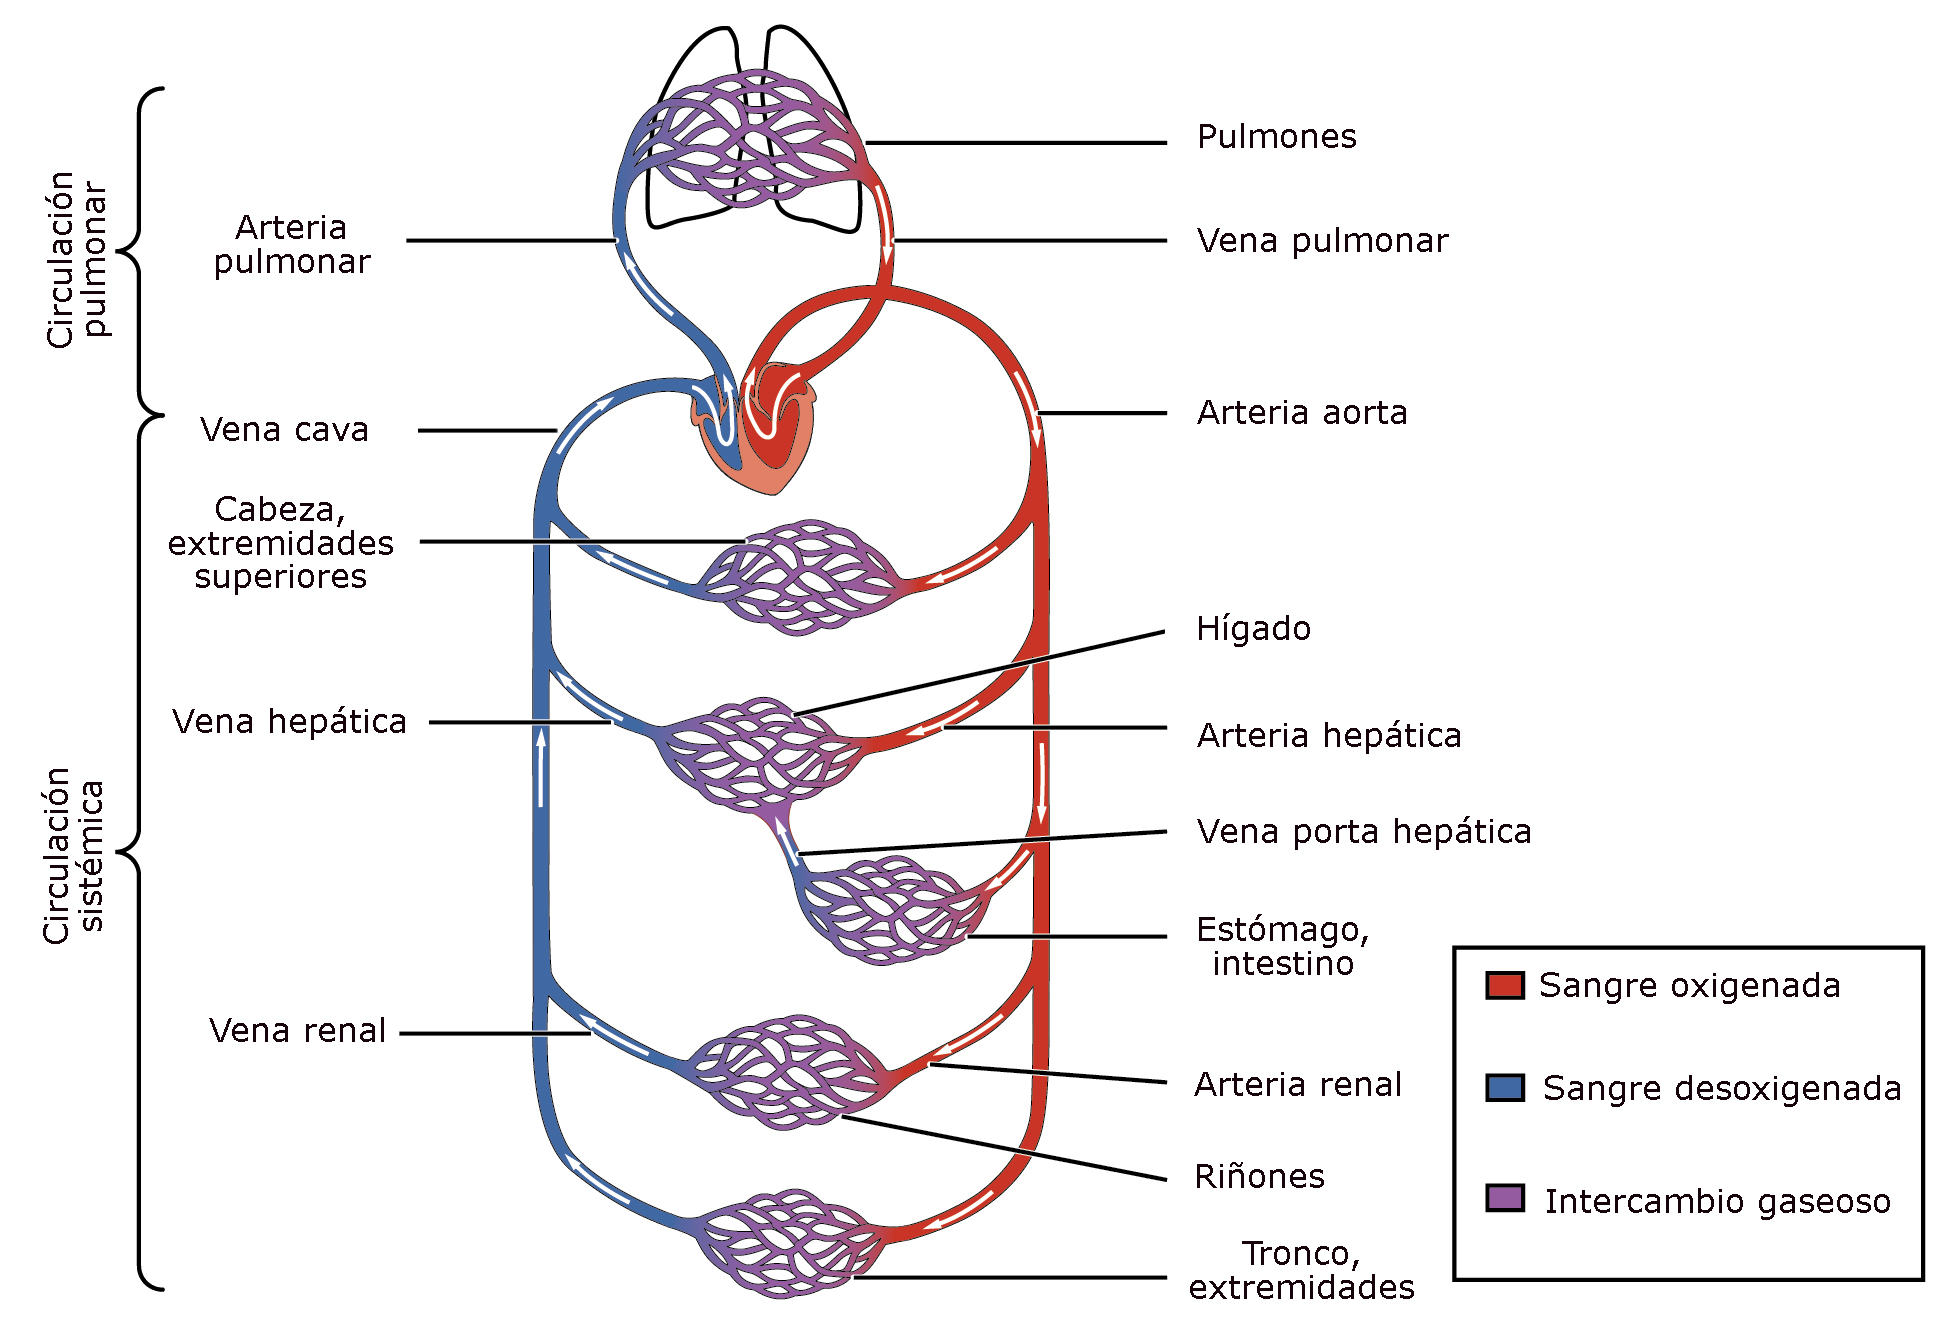
\includegraphics[scale=0.2]{figures/CicloSangre.jpg}
    \caption{El ciclo que cumple la sangre en el cuerpo humano. Imagen tomada de \cite{eswiki:159489943}.}
    \label{sec:RBC:fig:CicloSangre}
\end{figure}

Durante un periodo aproximado entre 90 y 120 días, unos tres o cuatro meses, los nuevos glóbulos rojos completan el ciclo cardíaco gracias a los bombeos del corazón, viajando de los pulmones, para recibir el oxigeno, hasta todos lo órganos, para entregarles el oxigeno y recibir el dióxido de carbono, como se ilustra en la figura \ref{sec:RBC:fig:CicloSangre}. De esta manera, hacer una observación de la población de glóbulos rojos diaria es acertado, pues su ciclo de vida es medido en días.

Al cumplir su vida útil, la membrana de los glóbulos rojos está debilitada y su tamaño reducido, por lo que los eritrocitos pueden ser filtrados por el bazo y eliminados por el cuerpo. También es posible que, al ser más frágiles de lo normal, los RBC's exploten dentro del torrente sanguíneo, pero las células macrófagas de la sangre son capaces de digerirlos rápidamente. Para calcular la cantidad de eritrocitos que mueren al día, basta hacer el cálculo de 25 trillones de RBC's entre 120 días que es la vida promedio de estos, obteniendo un resultado aproximado de 208 billones de glóbulos rojos eliminados diariamente.

Contando con todo el ciclo expuesto, un diagrama compartimental, basado en aquel que se presenta en \cite{kirk1968mathematical}, que puede mostrar claramente el ciclo de vida de los glóbulos rojos es el siguiente:

\begin{figure}[H]
    \centering
    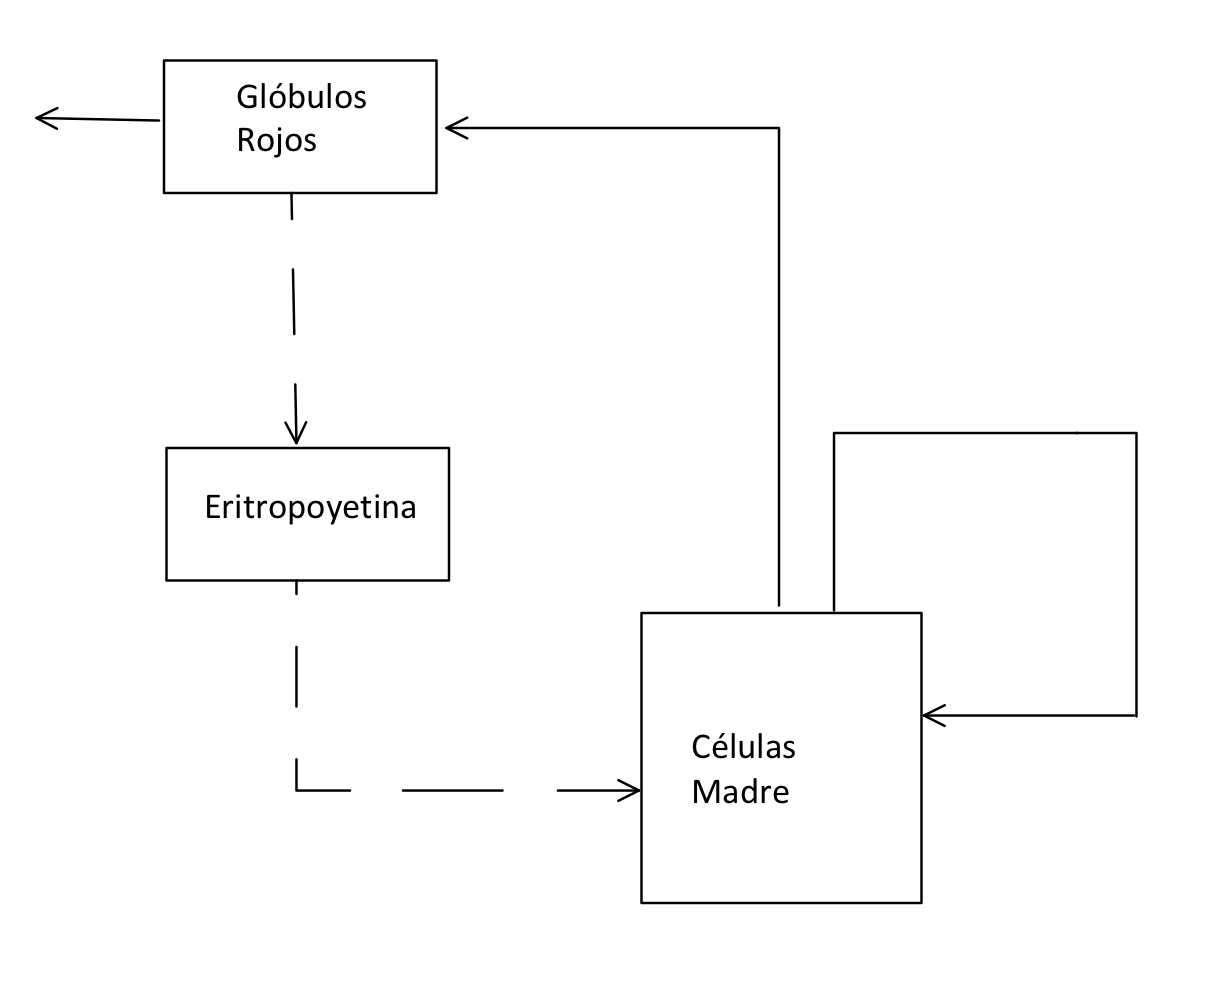
\includegraphics[scale=0.3]{figures/VidaRBC.jpeg}
    \caption{El proceso de producción y eliminación de glóbulos rojos.}
    \label{sec:RBC:fig:VidaRBC}
\end{figure}

En donde se desestima la transformación de células madre en otro tipo de células del cuerpo, fuera de la mitosis para autorreproducirse. La línea punteada implica que es bajo la acción de la eritropoyetina que las células madre reciben la señal de iniciar la eritropoyesis.

\section{Homeostasis}\label{sec:RBC:homeostasis}

Biológicamente, la \textbf{homeostasis} se define como la propiedad que tienen los organismos vivos de mantener un equilibrio estable al compensar pérdidas y ganancias. De esta manera, la hematología también es la encargada de estudiar la homeostasis de la sangre y de los glóbulos rojos en el cuerpo humano. Diferentes enfermedades o percances como la anemia, definida como el déficit de glóbulos rojos o de hemoglobina en la sangre, o las hemorragias deben de ser tenidas en cuenta para generar y simular un buen modelo matemático de las dinámicas de los glóbulos rojos en el cuerpo humano.

\section{Enfermedades y Complicaciones}\label{sec:RBC:enfermedades}

A la hora de construir un modelo matemático para las dinámicas de los glóbulos rojos, es importante considerar algunos factores externos que pueden perturbar la homeostasis como enfermedades o complicaciones médicas, pues no tener en cuenta estos factores hace que el modelo no sea realista. Para la presente investigación, se tendrán en cuenta la anemia y las hemorragias.

\subsection{Anemia}\label{subsec:RBC:enfermedades:anemia}
La \textbf{anemia}, siguiendo las definiciones de Portoles en \cite{portoles2021anemia} y de Heras en \cite{heras2023anemia}, es la deficiencia de hemoglobina en el cuerpo humano, para hombres esta se considera en valores menores a 13 gramos por decilitro de sangre y para mujeres en valores menores a 12 gramos por decilitro de sangre. Una de las variantes de la anemia es la \textbf{anemia renal}, se produce por deficiencia de eritropoyetina, de hierro o de otras sustancias importantes para la eritropoyesis que son sintetizadas por los riñones, esto quiere decir que la deficiencia de producción de glóbulos rojos es un factor importante a tener en cuenta para las causas de la anemia renal.

Los pacientes que sufren de anemia suelen presentar cansancio y falta de aire a causa de la deficiencia de oxígeno en el cuerpo, pues al no haber suficientes RBC's o hemoglobina, la cantidad de oxígeno transportada por medio de la sangre es mucho menor. Teniendo esto en cuenta, es importante resaltar que una anemia grave puede resultar mortal para el ser humano y que sumada a otras enfermedades, como la enfermedad renal crónica, puede resultar en problemas cardíacos, pues el corazón debe cambiar su funcionamiento para intentar mantener oxigenados los órganos.

Entre los posibles tratamientos para esta enfermedad está en el uso de agentes estimuladores de la eritropoyesis, como la eritropoyetina, el hierro y las transfusiones sanguíneas, ya que estos componentes son los que permiten el aumento de los glóbulos rojos en el cuerpo y, de esta manera, de la hemoglobina. Estos tratamientos, sin embargo, pueden tener efectos secundarios como complicaciones cardiovasculares o el aumento drástico del hierro en el cuerpo, que puede derivar en diabetes. La eritropoyetina se aplica mediante inyecciones subcutáneas (es decir en la piel) o directamente en una vena, para los pacientes con anemia renal se recomienda la aplicación de entre 50 y 100 unidades por kilogramo de masa corporal según la Mayo Clinic en \cite{MayoClinic}.

\subsection{Hemorragias}\label{subsec:RBC:enfermedades:hemorragias}
Una \textbf{hemorragia}, siguiendo las definiciones de Sánchez en \cite{Sanchez2000Hemorragias}, o sangrado, es la pérdida de sangre en el cuerpo, ya sea internamente o externamente. Las hemorragias tienen múltiples causas, como cortes o golpes, y son sumamente comunes entre los seres humanos. Las hemorragias leves, causadas por cortes superficiales o golpes suaves, no necesitan tratamiento, pues el mismo cuerpo es capaz de cerrar la herida para frenar el sangrado y recomponer los eritrocitos perdidos. Los sangrados fuertes, sin embargo, deben ser tratados con urgencia, pues la constante pérdida de grandes cantidades de sangre puede ocasionar graves complicaciones e, inclusive, la muerte. No hay cifras para diferenciar un sangrado leve de uno grave, pero es claro que si hay una gran o continua pérdida de sangre se debe actuar inmediatamente, pues puede ser causado por la ruptura de algún vaso sanguíneo importante o de algún órgano. Si un ser humano pierde cerca del $20\%$ de su cantidad habitual de sangre, esto puede causar un shock hipovolémico, es decir que los órganos empiezan a dejar de funcionar (\cite{PerdidaSangre}).

Los pacientes que han perdido mucha sangre pueden presentar, así como con los pacientes anémicos, un fuerte cansancio y dificultades para respirar, aunque también puede llegar a extremos como el mareo o los desmayos.

Para tratar una hemorragia grave se debe localizar la herida que la causa y tratarla inmediatamente, y para compensar la pérdida de sangre se debe hacer una transfusión sanguínea mediante vía intravenosa, que suele tardar entre 1 y 4 horas con bolsas de 250 mililitros de glóbulos rojos siguiendo las recomendaciones del centro de transfusión, tejidos y células de Granada en España en \cite{Granada}. 

Habiendo ya visto desde una perspectiva fisiológica las dinámicas de los glóbulos rojos en el cuerpo humano, se procederá a presentar y analizar un modelo matemático que intente imitar tales dinámicas.


% All contribution chapters should follow a similar structure, with a
% mini-introduction and overview at the beginning and a conclusion at the
% end bookmarking a structured presentation of the contribution. This can be
% largely based on your publications.

\chapter{Modelo Base}\label{chap:modelo}
\section{Introducción}\label{sec:modelo:intro}
Ya tieniendo en cuenta las dinámicas de los glóbulos rojos en el cuerpo humano, se procederá a analizar y simular el modelo matemático de estas propuesto por Eldestein \cite{edelstein2005} utlizando las técnicas presentadas en \ref{chap:Apendice}. 

Es importante tener en cuenta que el modelo que sea que se analice debe tener concordancia con la vida real en cuanto a las variables y a las constantes utilizadas. La homeostasis es fundamental en todo proceso biológio y es por eso que el modelo y las simulaciones deben reflejar correctamente el equilibrio del sistema. Adicionalmente, es clave considerar que es imposible lograr una formulación matemática que este totalmente en concordancia con todos los procesos biológicos que suceden dentro del cuerpo humano, pues se debería tener en consideración una enorme cantidad de variables, de actores y de estado que se salen del propósito básico de simplificar el problema. De esta manera, los modelos propuestos son un acercamiento aproximado a la realidad del problema.

\section{Presentación del Modelo}\label{sec:modelo:presentacion}
Considerando la elemincación de glóbulos rojos del bazo y su producción por la medula ósea para mantener la homeostasis y el diagrama de cajas de la figura \ref{sec:RBC:fig:VidaRBC}, el modelo propuesto por Eldestein es el siguiente:
$$R(n+1)=(1-f)R(n)+M(n),$$
$$M(n+1)=\gamma \cdot f\cdot R(n),$$

en donde $R=R(n)$ representa la cantidad de glóbulos rojos por mililitro de sangre y $M=M(n)$ la cantidad de glóbulos rojos por mililitro de sangre que prodeuce la médula ósea. $\gamma>0$ representa la cantidad de glóbulos rojos producida por cada uno perdido y $0\leq f \leq 1$ el porcentaje de glóbulos rojos por mililitro de sangre que elimina el bazo. Ni $\gamma$ ni $f$ tienen unidades dadas estas definiciones.

De esta manera, el modelo se puede interpretar de la siguiente manera: la cantidad de RBC's en el día $n+1$ ($R(n+1)$) es el porcentaje restante del día $n$ más lo que haya producido la médula ósea en el día $n$; mientras que la cantidad de eritrocitos producidos por la médula ósea en el día $n+1$ ($M(n+1)$) es un múltiplo de la cantidad de glóbulos rojos eliminada en el día $n$. Este modelo es una simplificación bastante acertada de lo visto en \ref{sec:RBC:fig:CicloSangre} en cuanto a la relación entre producción y eliminación de RBC's; es claro que para ser aún más acertados se podrían agregar muchas otras variables como el funcionamiento de los riñones para la producción de eritropyetina, el proceso de absorción del hierro o la edad y estado de salud del sujeto analizado, pero estos complican innecesariamente el modelo y su análisis.

\section{Análisis del Modelo}\label{sec:modelo:analisis}
Ahora se procederá a analizar las soluciones del modelo a través de los métodos de ecuaciones en diferencias y de la matriz resultante del modelo.
\subsection{Método mediante Ecuaciones en Diferencias}

Nótese que las ecuaciones del modelo se pueden reducir a una única ecuación en términos de $R(n)$ de la siguiente manera:
$$M(n)=\gamma f R(n-1)$$
$$\implies R(n+1)=(1-f)R(n)+\gamma f R(n-1)$$
$$\implies R(n+2)=(1-f)R(n+1)+\gamma f R(n)$$
$$\implies R(n+2)-(1-f)R(n+1)-\gamma f R(n)=0.$$

Esta ecuación se puede tomar como una ecuación en diferencia homogenea lineal de grado 2, por lo que se pueden hallar sus soluciones al encontrar las raíces del polinomio característico de la ecuación:
$$p(\lambda)=\lambda^2-(1-f)\lambda-\gamma f$$
$$\implies \lambda_{1,2}=\dfrac{(1-f)\pm\sqrt{(1-f)^2+4\gamma f}}{2}.$$

Dado que $0\leq f \leq 1$ y $\gamma > 0$, entonces el radicando será positivo, por lo que los valores $\lambda_{1,2}$ son números reales, y de esta manera la solución general de la ecuación en diferencias es de la forma:
$$R(n)=c_1 \lambda_1^n+ c_2 \lambda_2^n,$$
en donde $c_{1,2}$ dependerán de las condiciones iniciales que se utilicen.

\subsection{Método mediante Matrices}

La matriz resultante del modelo es:
$$X_{n+1}=\begin{pmatrix}
    R(n+1) \\
    M(n+1) 
    \end{pmatrix}=
    \begin{pmatrix}
    1-f & 1\\
    \gamma f & 0 
    \end{pmatrix} \cdot 
    \begin{pmatrix}
    R(n) \\
    M(n) \\
    \end{pmatrix}=
    \begin{pmatrix}
        1-f & 1\\
        \gamma f & 0 
        \end{pmatrix} X_n,$$

por lo que para el ánalisis de soluciones se debe estudiar la matriz
$$A=\begin{pmatrix}
    1-f & 1\\
    \gamma f & 0 
    \end{pmatrix}.$$

Los autovalores de $A$ se obtienen al calcular las solciones $\lambda_{1,2}$ del determinante de $A-\lambda I$:
$$det(A-\lambda I) = \begin{vmatrix}
    1-f-\lambda & 1\\
    \gamma f & -\lambda 
    \end{vmatrix} = -\lambda(1-f-\lambda)-\gamma f$$

$$=\lambda^2-(1-f)\lambda-\gamma f,$$

utilizando la fórmula cuadrática, se obtiene
$$\lambda_{1,2}=\dfrac{(1-f)\pm\sqrt{(1-f)^2+4\gamma f}}{2}.$$

Los vectores propios correspondientes a estos valores propios son los vectores $\mathbf{v_{1,2}}$ que solucionan la ecuación
$$(A-\lambda_i I)\mathbf{v_i}=0, \:\:\: i=1,2,$$

y de esta manera la solución general del problema estará dada por

$$\begin{pmatrix}
    R(n) \\
    M(n) 
    \end{pmatrix}= (\lambda_1)^n \mathbf{v_1}+(\lambda_2)^n \mathbf{v_2}.$$


Nótese que ambos métodos, al arrojar el mismo polinomio característico, obtienen la misma solución general del sistema, esto implica que el modelo propuesto está bien fundamentado matemáticamente.

\section{Derivación de Parámetros y Análisis}\label{sec:modelo:parametros}
Para poder pasar a valores específicos de las soluciones encontradas, es necesario dar valores numéricos a los parámetros $\lambda$ y $f$, pues el modelo depende de estos y, junto a las condiciones iniciales, determinan las soluciones del problema. Para hallar estos parámetros, se utilizará la información brindada en \ref{sec:RBC:vida} sobre la producción de glóbulos rojos a través de la médula ósea y de su eliminación por medio del bazo.

Inicialmente, es necesario declarar las condiciones iniciales del problema. Dado que las solcuines encontradas dependen, en el caso de ecuaciones en diferencia, de dos constantes o, en el caso de matrices, de dos vectores, es necesario que hayan dos condiciones iniciales del problema: $R(0)$ y $R(1)$ o $X_0$. $R(0)$ representa la cantidad de glóbulos rojos al momento inicial de la medida, que se tomará como 125 trillones ($25\times 10^{12}$). Para el caso de la matriz, se puede tomar que $R(0)$ se mantiene como en el caso anterior y tomar $M(0)=0$, pues el instante que se inicia la medición, el cuerpo no ha generado nuevos glóbulos rojos. $M(0)$, como se verá más adelante en las simulaciones, es un valor muy interesante a tener en cuenta y que modifica relativamente los resultados obtenidos, pues al considerar o no que la médula ósea ha producido RBC's al momento de la primera medición, $R(1)$ cambiará.

Ahora, determinar $f$ es relativamente sencillo, pues es el porcentaje diario de RBC's que elimina el cuerpo. Contando con que la cantidad promedio es de eritrocitos es de $25\times 10^{12}$ y que diariamente mueren $208\times 10^{9}$, entonces el porcentaje de glóbulos rojos elminados diariamente por el bazo es del $0.832\%$, es decir que se puede tomar $f=0.00832$. 

Determinar el valor biológico de $\gamma$ es mucho más complicado, pues no ha sido posible determinar la cantidad de glóbulos rojos que produce una célula madre durante la eritropoyesis. Para hallar un valor adecuado de $\gamma$, se hará el análisis matemático y de las simulaciones con los valores ya establecidos. En todo caso, se puede hace el análisis para los diferentes casos:
\begin{enumerate}
    \item  $\gamma<1$: Este caso implica que el cuerpo produce una menor cantidad de eritrocitos respecto a la que elimina, por lo que los resultados deberían mostrar una caída en la cantidad de glóbulos rojos.
    \item $\gamma=1$: Este caso implica que el cuerpo produce la misma cantidad de eritrocitos respecto a la que elimina, por lo que los resultados deberían mostrar una estabilidad en la cantidad de glóbulos rojos.
    \item  $\gamma>1$: Este caso implica que el cuerpo produce una mayor cantidad de eritrocitos respecto a la que elimina, por lo que los resultados deberían mostrar un crecimiento en la cantidad de glóbulos rojos.
\end{enumerate}

En el caso esperado, es decir en el que el cuerpo alcanza la homeostasis, el valor deseado de $\gamma$ es $1$, pues de esta manera el cuerpo no pierde células, ya que todas aquellas que mueren son producidas. En todo caso, las simulaciones que se hagan utilizarán variaciones en este parámetro.

Como ya se ha visto en \ref{sec:modelo:analisis}, las soluciones del problema dependen de las constantes y de los valores iniciales, a continuación se calcularán las soluciones bajo los valores derivados para cada parámetro: $\gamma = 1$, $f = 0.00832$, $R(0)=25\times 10^{12}$, $M(0)=208\times 10^{9}$ 

\begin{itemize}
    \item Para el caso de ecuaciones en diferencias, se obtiene que las soluciones del polinomio carácterístico de la ecuación son:
        $$\lambda_{1,2}=\dfrac{(1-f)\pm\sqrt{(1-f)^2+4\gamma f}}{2}$$
        $$=\dfrac{(1-0.00832)\pm \sqrt{(1-0.00832)^2+4(0.00832)}}{2}$$
        $$\implies \lambda_1 = 1,\;\;\; \lambda_2 = -0.00832=-f.$$
        Y así, la solución general está dada por 
        $$R(n)=c_1+c_2(-0.00832)^n$$
        $$R(0)=25\times 10^{12}=c_1+c_2$$
        $$R(1)=(1-f)R(0)+M(0)=(1-0.00832)25 \times 10^{12}+208\times 10^9$$
        $$=c_1-0.00832\cdot c_2,$$
        resolviendo el sistema $2\times 2$ conformado por $c_{1,2}$ se obtienen los resultados $c_1=25\times 10^{12}$, $c_2 = 0$. Lo que quiere decir que la solución del problema, dadas las condiciones iniciales es:
        $$R(n)=25\times 10^{12},$$
        como es esperado, pues obtener una solución constante implica que el cuerpo logra mantener la homeostasis, es decir que en ningún momento hay pérdias o ganancias de RBC's en el cuerpo.
    \item En el caso de utilizar la matriz que representa el modelo, los valores propios hallados son
        $$\lambda_1 = 1, \;\;\; \lambda_2 = -0.00832=-f,$$
        mientras que los vectores propios asociados a cada valor propio son (aproximando a 4 cifras significativas):
        $$\mathbf{v_1}=\begin{pmatrix}
            0.9999  \\
            -0.7071
            \end{pmatrix},\;\;\;  \mathbf{v_2}=\begin{pmatrix}
            0.0083 \\
            0.7071
            \end{pmatrix}.$$

\end{itemize}

Considerando el caso $\gamma = 0.7$, las soluciones son las siguientes:
\begin{itemize}
    \item Para el caso de ecuaciones en diferencias, se obtiene que las soluciones del polinomio carácterístico de la ecuación son (aproximando a 4 cifras significativas):
        $$\lambda_1 = 0.9975,\;\;\; \lambda_2 = -0.0058.$$
        Y así, la solución general está dada por 
        $$R(n)=c_1(0.9975)^n+c_2(-0.0058)^n$$
        resolviendo el sistema $2\times 2$ conformado por $c_{1,2}$ se obtienen los resultados $c_1=25.0618\times 10^{12}$, $c_2 = -61.8302\times 10^{9}$. Lo que quiere decir que la solución del problema, dadas las condiciones iniciales es:
        $$R(n)=(25.0618\times 10^{12})(0.9975)^n+(-61.8302\times 10^{9})(-0.0058)^n,$$
        nótese que en este caso el valor absoluto de los valores propios son ambos menores a 1, esto quiere decir que entre más tiempo avance, al elevar estos valores a la $n$-ésima potencia, la solución se acercará al 0. Esto quiere decir que, como se esperaba, hay una pérdida en la cantidad de glóublos rojos con el paso del tiempo.
    \item En el caso de utilizar la matriz que representa el modelo, los valores propios hallados son (aproximando a 4 cifras significativas):
        $$\lambda_1 = 0.9975, \;\;\; \lambda_2 = -0.0058,$$
        mientras que los vectores propios asociados a cada valor propio son (aproximando a 4 cifras significativas):
        $$\mathbf{v_1}=\begin{pmatrix}
            0.9999  \\ 
            -0.7079
            \end{pmatrix},\;\;\;  \mathbf{v_2}=\begin{pmatrix}
            0.0058  \\
            0.7062
            \end{pmatrix}.$$

\end{itemize}

Considerando el caso $\gamma = 1.3$, las soluciones son las siguientes:
\begin{itemize}
    \item Para el caso de ecuaciones en diferencias, se obtiene que las soluciones del polinomio carácterístico de la ecuación son (aproximando a 4 cifras significativas):
        $$\lambda_1 = 1.0025,\;\;\; \lambda_2 = -0.0108.$$
        Y así, la solución general está dada por 
        $$R(n)=c_1(1.0025)^n+c_2(-0.0108)^n$$
        resolviendo el sistema $2\times 2$ conformado por $c_{1,2}$ se obtienen los resultados $c_1=24.9391\times 10^{12}$, $c_2 = 60.9261\times 10^{9}$. Lo que quiere decir que la solución del problema, dadas las condiciones iniciales es:
        $$R(n)=(24.9391\times 10^{12})(1.0025)^n+(c_2 = 60.9261\times 10^{9})(-0.0108)^n,$$
        nótese que en este caso $\lambda_1>1$ y $|\lambda_2|<1$, esto quiere decir que entre más tiempo avance, al elevar estos valores a la $n$-ésima potencia el adendo con $\lambda_1$ crecerá hacia el inifinito mientras que el de $\lambda_2$ caerá hacia el 0. Esto quiere decir que, como se esperaba, hay un aumento en la cantidad de glóublos rojos con el paso del tiempo.
    \item En el caso de utilizar la matriz que representa el modelo, los valores propios hallados son (aproximando a 4 cifras significativas):
        $$\lambda_1 = 1.0025, \;\;\; \lambda_2 = -0.0108,$$
        mientras que los vectores propios asociados a cada valor propio son (aproximando a 4 cifras significativas):
        $$\mathbf{v_1}=\begin{pmatrix}
            0.9999  \\ 
            -0.7062
            \end{pmatrix},\;\;\;  \mathbf{v_2}=\begin{pmatrix}
            0.0108  \\
            0.7079
            \end{pmatrix}.$$

\end{itemize}

\section{Simulaciones}\label{sec:modelo:simulaciones}
A continuación se presentarán las simulaciones computacionales del modelo y su respectivo análisis según los valores escogidos de $\gamma$. Es importante apuntar que cada una de las simulaciones considera el tiempo de 10 días.

Para cada una de las simulaciones, estos valores son fijos:
\begin{itemize}
    \item $f=0.00832$;
    \item $R(0) = 25\times 10^{12};$
    \item $M(0) = 208 \times 10^{9}.$
\end{itemize}

\subsection{Caso $\gamma=1$}
\begin{figure}[H]
    \centering
    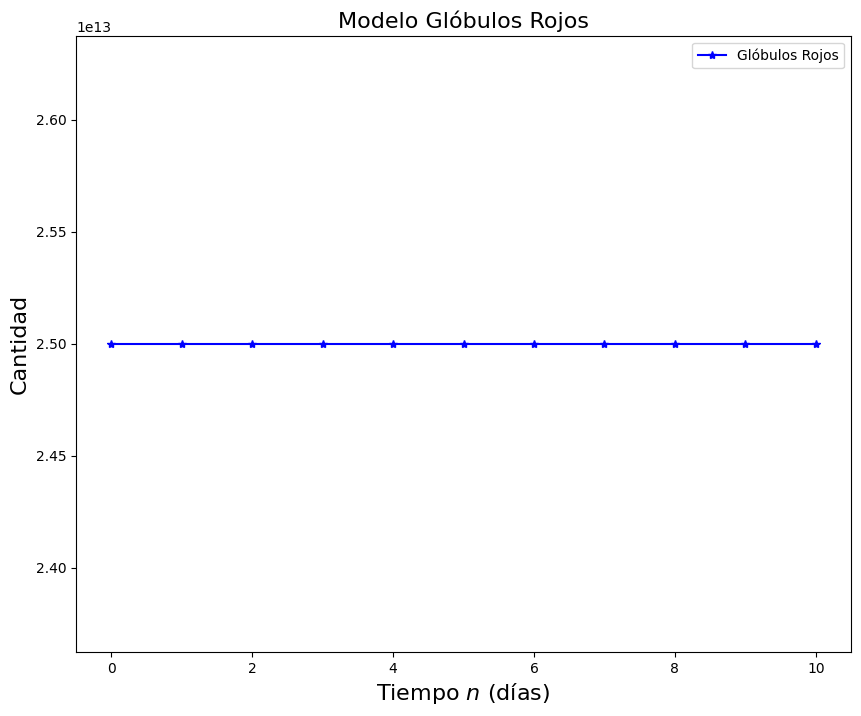
\includegraphics[scale=0.55]{figures/BaseG1RBC.png}
    \caption{Caption?}
    \label{sec:modelo:fig:G1RBC}
\end{figure}

\begin{figure}[H]
    \centering
    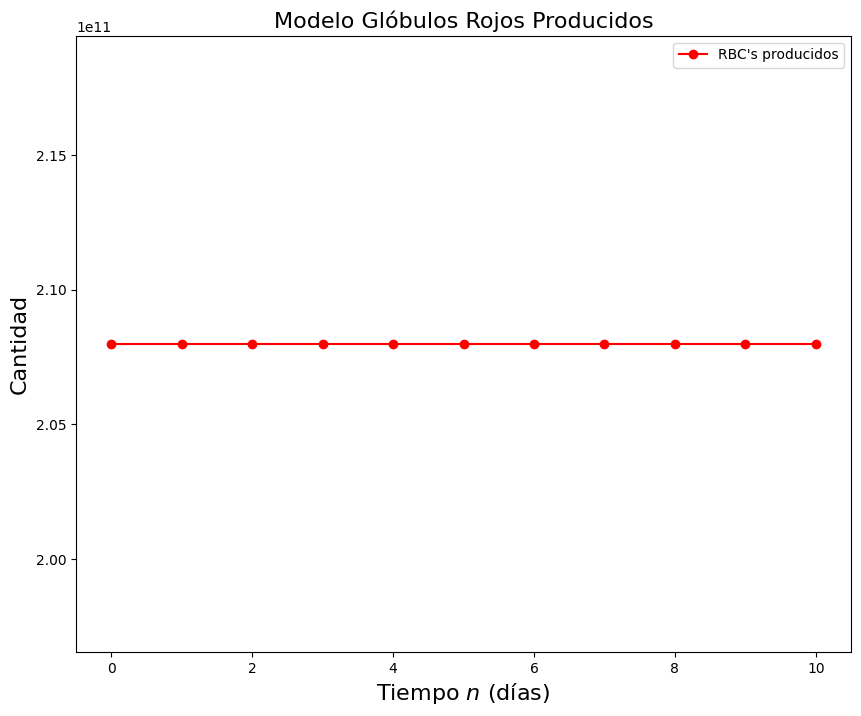
\includegraphics[scale=0.55]{figures/BaseG1SC.png}
    \caption{Caption?}
    \label{sec:modelo:fig:G1SC}
\end{figure}
Como era esperado, según los análisis hechos en \ref{sec:modelo:analisis}, para el caso $\gamma = 1$ se obtiene una simulación totalmente estable, manteniendo el nivel de glóbulos rojos diarios en $25\times 10^{12}$ y la cantidad de glóbulos rojos producidos diariamiente en $208\times 10^{9}$. Esta simulación representa el caso ideal en el que un paciente no tenga ninguna enfermedad o complicación médica y sea completamente saludable. Para este caso, todo glóbulo rojo que es eliminado por el bazo es producido por la médula ósea, por lo que no hay variaciones en las cantidades.

\subsection{Caso $\gamma=0.7$}
\begin{figure}[h]
    \centering
    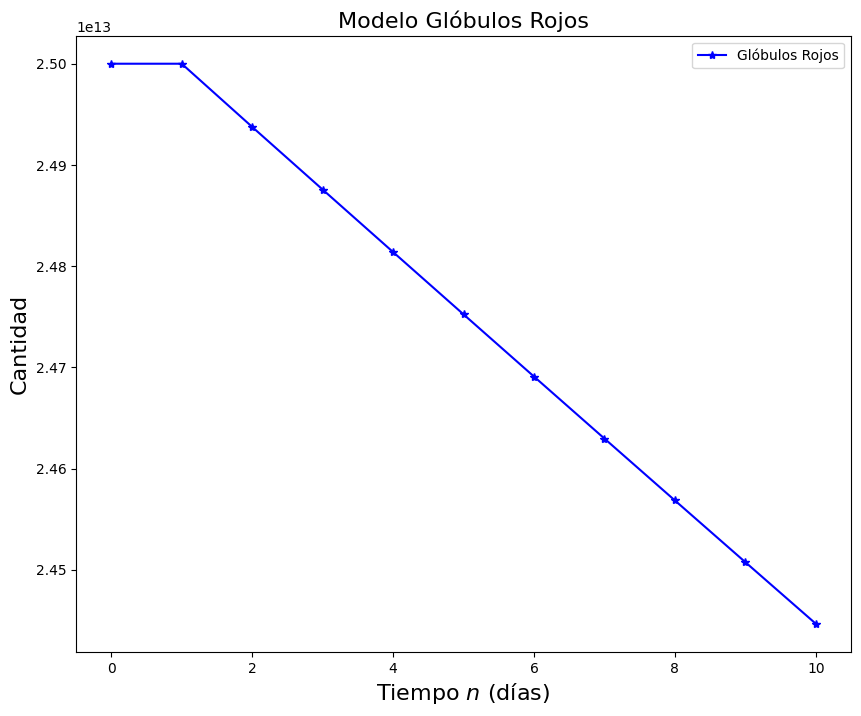
\includegraphics[scale=0.55]{figures/BaseG07RBC.png}
    \caption{Caption?}
    \label{sec:modelo:fig:G07RBC}
\end{figure}

En este caso, el paciente padece de una enfermedad que afecta la producción de glóbulos rojos producidos por la médula ósea, pues $\gamma=0.7$ implica que por cada glóbulo rojo eliminado por el bazo se producen únicamente $0.7$ glóbulos rojos. Como se puede observar en las simulaciones, los efectos de una baja producción de RBC's es una caída tanto en la cantidad de eritrocitos en el cuerpo como en su producción por parte de las células madre. Extendiendo los días simulados se encuentra que en el día 280 la cantidad de glóbulos rojos se ha reducido a la mitad respecto a la inicial. Un aspecto interesante es la caída que se puede obervar en la figura \ref{sec:modelo:fig:G07SC} y la estabilidad en la figura \ref{sec:modelo:fig:G07RBC} del día 0 al día 1, pero esta ocurre dado que las condiciones iniciales asumen que en el día 0 la producción es normal y a partir del día 1 es que ocurre el cambio en la producción de RBC's, por lo que ahí ocurre la primera caída en producción y en cantidad. 

\begin{figure}[h]
    \centering
    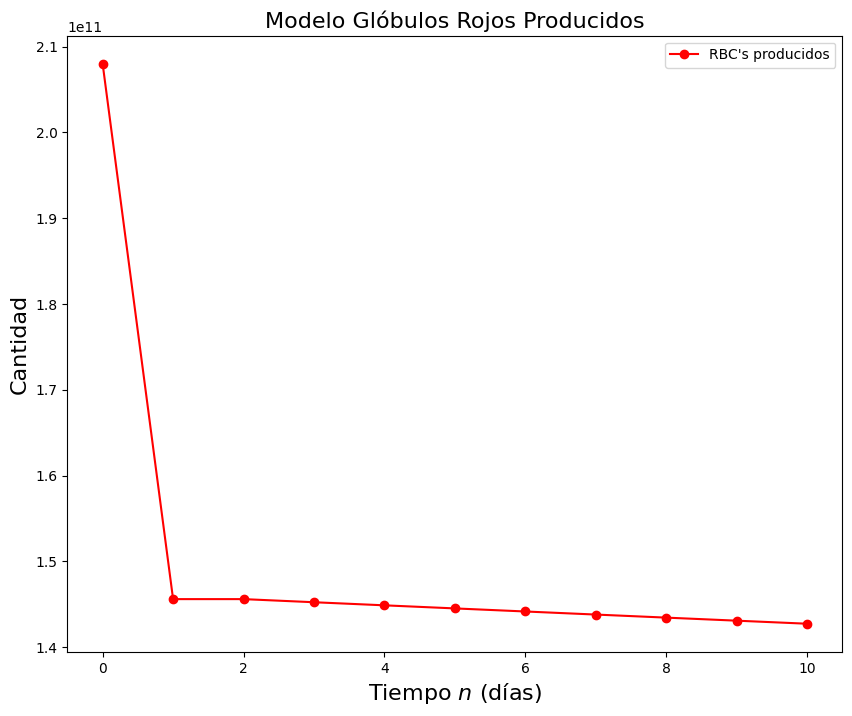
\includegraphics[scale=0.55]{figures/BaseG07SC.png}
    \caption{Caption?}
    \label{sec:modelo:fig:G07SC}
\end{figure}

\FloatBarrier

\subsection{Caso $\gamma=1.3$}

\begin{figure}[h]
    \centering
    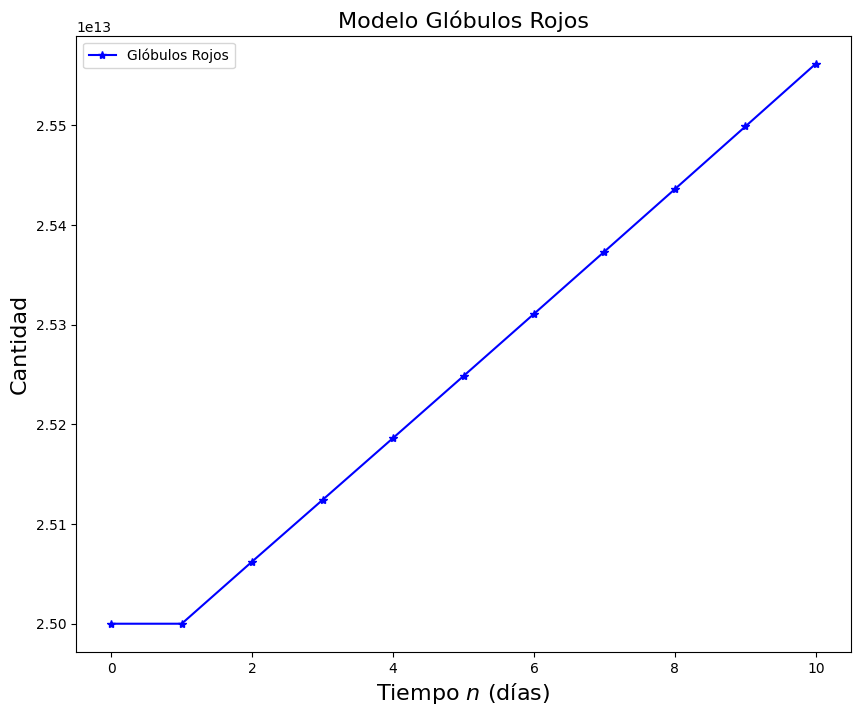
\includegraphics[scale=0.55]{figures/BaseG13RBC.png}
    \caption{Caption?}
    \label{sec:modelo:fig:G07RBC}
\end{figure}

\begin{figure}[h]
    \centering
    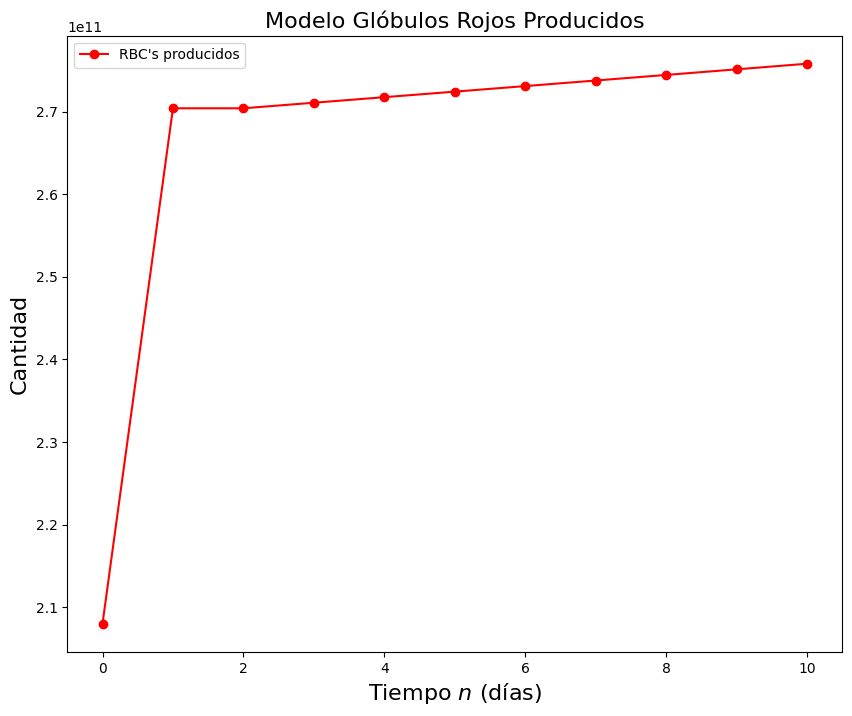
\includegraphics[scale=0.55]{figures/BaseG13SC.png}
    \caption{Caption?}
    \label{sec:modelo:fig:G07SC}
\end{figure}

\chapter{Variaciones del Modelo}\label{chap:variaciones}

Teniendo ya claros los conceptos médicos y el análisis de un modelo base acorde con tales conceptos, es momento de introducir al modelo las dos enfermedades presentadas en la sección \ref{sec:RBC:enfermedades}: el caso de las hemorragias y el de la anemia. Los sangrados son tratados una única vez (hasta que sean frenados), mientras que la anemia es una enfermedad cuyo tratamiento es para toda la vida. En este capítulo se presentarán las variaciones matemáticas del modelo y el análisis de las simulaciones de estas variaciones, esperando que los resultados obtenidos logren mantener la homeostasis del paciente y, para el caso de la anemia, ver si un aumento o disminución de la dosis afecta realmente los resultados.

\section{Caso con Hemorragia}\label{Sec:variaciones:hemorragia}

Para los sangrados, se tendrán en cuenta diferentes casos. Inicialmente se tendrá en cuenta una hemorragia leve (pérdida del 2$\%$ de sangre) y se observará lo que sucede si, después de la pérdida de sangre, las variables del modelo se mantienen iguales y que sucede si estas se modifican. Posteriormente se considerará el caso de una hemorragia grave (el 14$\%$ de la sangre del cuerpo, que Holland lo considera grave pero no fatal en \cite{PerdidaSangre}) y se observarán los efectos de una transfusión sanguínea para recuperar la homeostasis. En el caso de las hemorragias, se tendrá en cuenta el caso en el que $\gamma =1$, pues así el paciente es totalmente sano, el parámetro $f$ se mantiene igual que antes ($=0.00832$) y los valores iniciales también se mantienen.

\subsection{Hemorragia Leve}\label{subsec:variaciones:hemorragia:leve}

Para esta variación del modelo, tome como ejemplo que en el tercer día de medición el paciente, ya sea por un corte o un accidente, pierde el $2\%$ de su cantidad de sangre en el cuerpo que, considerando el caso de que tenga 5 litros de sangre, esto equivale a 100 mililitros de fluido o a $5\times 10^{11}$ glóbulos rojos. Así, el modelo se puede ver de la siguiente manera:

\begin{align}\label{eq:HemoLeveMal}
    R(n+1) &= \left\{ \begin{array}{lcc} (1-f)\cdot R(n)+M(n) & \textrm{si} & n \neq 3 \\ \\ (1-f)\cdot R(n)+M(n)-0.02\cdot R(n) & \textrm{si} & n = 3\end{array} \right., \\
    M(n+1) &=\gamma \cdot f \cdot R(n). \nonumber
\end{align}

En donde:
\begin{itemize}
    \item $\gamma=1$; (glóbulos rojos producidos por cada uno perdido)
    \item $f=0.00832$; (fracción de glóbulos rojos eliminados diariamente)
    \item $R(0) = 25\times 10^{12}$; (cantidad inicial de glóbulos rojos)
    \item $M(0) = 208 \times 10^{9}$. (RBC's eliminados por la médula ósea en el día 0)
\end{itemize}

La simulación se ve así: en la primera gráfica de la figura \ref{sec:variaciones:fig:HemoLeveG1} se observa la pérdida de RBC's en el tercer día, un aumento en la cantidad de eritrocitos del tercero al cuarto y estabilidad del cuarto en adelante. En la segunda gráfica se observa lo mismo pero con un día de atraso. El aumento de RBC's que se puede observar está dado por el hecho de que el adendo $M(n)$ conserva lo que ha ocurrido en $R(n-1)$ así, para el cuarto día se producen la cantidad de eritrocitos que se vienen produciendo regularmente antes del accidente, y desde el cuarto día en adelante este adendo ya se acomoda a la nueva cantidad de sangre. La estabilidad en los glóbulos rojos que se observa del cuarto día en adelante está dada por el hecho de que $\gamma = 1$. El modelo, de esta manera, funciona como lo hace normalmente (véase la sección \ref{subsec:modelo:simulaciones:G1}) tomando una cantidad inicial de sangre menor que la original, es decir que mantiene una estabilidad con la cantidad de RBC's del cuarto día, que es de $24.504\times 10^{12}$ glóbulos rojos. 

\begin{figure}[H]
    \centering
    \captionsetup{justification=centering}
    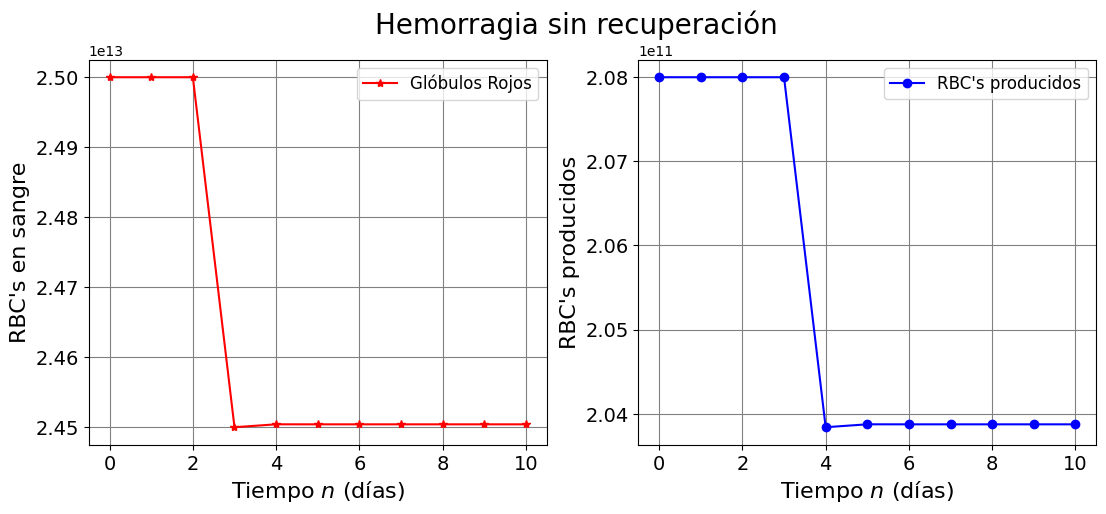
\includegraphics[scale=0.534]{figures/HemoLeveG1.png}
    \caption{Simulación del modelo para el caso de una hemorragia sin recuperación de la homeostasis. A la izquierda está la gráfica de $R(n)$, a la derecha la de $M(n)$.}
    \label{sec:variaciones:fig:HemoLeveG1}
\end{figure}

Está claro que esta simulación está totalmente alejada de lo que ocurre en el caso real, pues lo esperado es que el cuerpo recupere con el paso del tiempo la cantidad de glóbulos rojos perdidos, esto quiere decir que para $n>3$ se debe aumentar el valor de $\gamma$ hasta que la cantidad de eritrocitos sea mayor o igual a la inicial, es decir:

\begin{align}\label{eq:HemoLeveBien}
    R(n+1) &= \left\{ \begin{array}{lcc} (1-f)\cdot R(n)+M(n) & \textrm{si} & n \neq 3 \\ \\ (1-f)\cdot R(n)+M(n)-0.02\cdot R(n) & \textrm{si} & n = 3\end{array} \right. \\
    M(n+1) &=\left\{ \begin{array}{lcc} f\cdot \gamma_1 \cdot R(n) & \textrm{si} & R(n+1) \geq R(0) \\ \\ f\cdot \gamma_2\cdot R(n) & \textrm{si} & R(n+1)<R(0)\end{array} \right. \nonumber
\end{align}

La condición de $M(n+1)$ permite evitar el retraso del que se ha hablado anteriormente, pues si se considera que ya se alcanzó la cantidad ``normal'' de eritrocitos entonces el cuerpo no debe producir más de los necesarios.

Para calibrar el valor de $\gamma_2$ se utilizó la información brindada por el hospital general de Massachusetts en \cite{Massachusetts}, dado que al cuerpo le toma recuperar los glóbulos rojos perdidos en 450 ml de sangre en unas 5 semanas (35 días), entonces 100 ml deben recuperarse en unos 8 días. Las simulaciones hechas muestran que $\gamma=1.305$ permite lograr esta recuperación en ese tiempo.

Así, los valores constantes a tener en cuenta son:
\begin{itemize}
    \item $\gamma_1=1$; (glóbulos rojos producidos por cada uno perdido normalmente)
    \item $\gamma_2=1.305$; (glóbulos rojos producidos por cada uno perdido después de la hemorragia)
    \item $f=0.00832$; (fracción de glóbulos rojos eliminados diariamente)
    \item $R(0) = 25\times 10^{12}$; (cantidad inicial de glóbulos rojos)
    \item $M(0) = 208 \times 10^{9}$. (RBC's eliminados por la médula ósea en el día 0)
\end{itemize}

Para estas simulaciones, se utilizó un tiempo de 15 días para poder observar lo que sucede después de recuperar los eritrocitos perdidos:

\begin{figure}[H]
    \centering
    \captionsetup{justification=centering}
    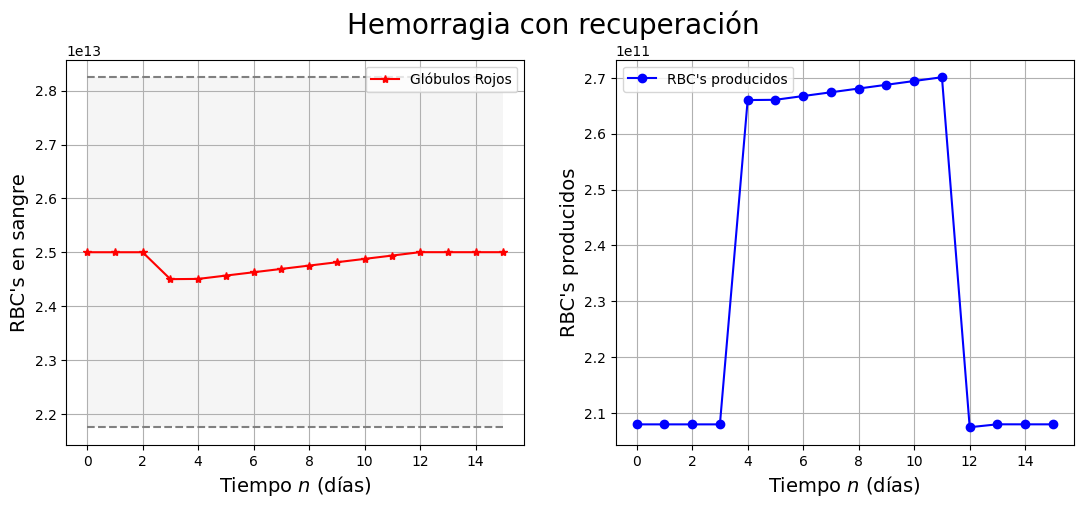
\includegraphics[scale=0.534]{figures/HemoLeveG13.png}
    \caption{Simulación del modelo para el caso de una hemorragia con recuperación de la homeostasis. A la izquierda está la gráfica de $R(n)$, a la derecha la de $M(n)$.}
    \label{sec:variaciones:fig:HemoLeveG13}
\end{figure}

Lo que se puede ver en estas gráficas es como, a partir del cuarto día (dado el retraso que presenta el modelo) se hace efectivo el cambio de $\gamma_1$ a $\gamma_2$, que se evidencia por el aumento en la primera gráfica de la figura \ref{sec:variaciones:fig:HemoLeveG13} del cuarto al duodécimo día y en la segunda gráfica del cuarto al undécimo día. En el día 12 es en el que por fin se ha superado (o igualado) la cantidad inicial de glóbulos rojos en el cuerpo, el aumento desde la pérdida muestra lo ilustrado en la sección \ref{subsec:modelo:simulaciones:G13}, donde hay un aumento constante de eritrocitos. Después de recuperar la cantidad de sangre perdida, el cuerpo vuelve a estabilizar su sistema, pues ha llegado a la homeostasis. La diferencia en la segunda gráfica de los días 0 a 3 y de los días 13 a 15 se debe a que ha aumentado la cantidad estable de sangre, y para compensar la pérdida el cuerpo debe producir más células.

Teniendo esto en cuenta, ahora se debe analizar el caso en el que el paciente sufre de una hemorragia más grave y debe ser sometido a una transfusión sanguínea para que pueda recuperarse.

\subsection{Hemorragia Grave}

Considérese el caso en el que el paciente analizado sufre, por ejemplo, una pérdida del 14$\%$ del volumen de sangre de su cuerpo (unos 700 mililitros o 3.25$\times 10^{12}$ eritrocitos) a causa de un accidente, ya sea una hemorragia interna causada por un golpe o una herida externa como un corte. Esta pérdida de sangre, según Holland en \cite{PerdidaSangre}, se puede considerar como grave pero no crítica (no tiene efectos secundarios mayores), por lo que este ejemplo debe ser tratado médicamente mediante una transfusión sanguínea y no afectará las dinámicas normales del cuerpo.

Dado que las bolsas de transfusión de glóbulos rojos tienen un volumen aproximado de 250 mililitros (\cite{Granada}), correspondiente al 5$\%$ de la concentración normal, unos 1.25$\times 10^{12}$ RBC's, entonces para subsanar la pérdida del 14$\%$ se tomará como ejemplo que le son suministradas al paciente dos bolsas de eritrocitos y el volumen restante podrá ser recuperado por el cuerpo.

Para poder adecuar el modelo al problema, se considerará que el sangrado inicia y termina en el tercer día y el suministro de sangre ocurre y finaliza en el cuarto. Para la presente investigación es útil definir este caso de tal manera para poder ilustrar correctamente las ecuaciones. Es importante notar que el cuerpo tendrá tres estados diferentes durante este caso: la estabilidad antes y después de la recuperación, el estado del día en el que se hace la transfusión y el estado de los días después de la transfusión. De esta manera, el cuerpo debe modificar su producción interna de RBC's en tres momentos, generando dos valores nuevos de $\gamma$ para cada cantidad de glóbulos rojos.

Así, una hemorragia grave se puede interpretar con la siguiente modificación del modelo base:

\begin{align}\label{eq:HemoGrave}
    R(n+1) &= \left\{ \begin{array}{lcc} (1-f)\cdot R(n)+M(n) & \textrm{si} & n \neq 3,4 \\ \\ (1-f)\cdot R(n)+M(n)-0.14\cdot R(n) & \textrm{si} & n = 3 \\ \\ (1-f)\cdot R(n)+M(n)+0.1\cdot R(0) & \textrm{si} & n = 4 \\ \end{array} \right. \\
    M(n+1) &=\left\{ \begin{array}{lcc} f\cdot \gamma_1 \cdot R(n) & \textrm{si} & R(n+1) \geq R(0) \\ \\ f\cdot \gamma_2\cdot R(n) & \textrm{si} & n = 4\textrm{ y } R(n+1)<R(0) \\ \\ f\cdot \gamma_3\cdot R(n) & \textrm{si} & n \neq 4\textrm{ y } R(n+1)<R(0)\\ \end{array} \right. \nonumber
\end{align}

Los valores de $\gamma_2$ y $\gamma_3$ fueron estimados al igual que en el caso de hemorragias leves. La cantidad de glóbulos rojos perdida en 700 mililitros de sangre debería ser recuperada por el cuerpo en unos 55 días, obteniendo un valor de $\gamma_2$ de 1.331. Para calibrar $\gamma_3$ se debe tener en cuenta la cantidad de eritrocitos en el cuerpo en el quinto día, pues el cuerpo del paciente se ajusta a la nueva cantidad de glóbulos rojos obtenidos gracias a la transfusión. En el quinto día de simulación, el cuerpo tiene 24.0673$\times 10^{12}$ RBC's, siguiendo la cuenta del hospital general de Massachusetts (\cite{Massachusetts}), la cantidad restante (93.2713 $\times 10^{10}$ eritrocitos) se recuperaría en 15 días, se concluye que $\gamma_3 = 1.31$ según las simulaciones del modelo.

Así, los valores constantes a tener en cuenta son:
\begin{itemize}
    \item $\gamma_1=1$; (glóbulos rojos producidos por cada uno perdido normalmente)
    \item $\gamma_2=1.305$; (glóbulos rojos producidos por cada uno perdido después de la hemorragia)
    \item $\gamma_3=1.31$; (glóbulos rojos producidos por cada uno perdido después de la transfusión)
    \item $f=0.00832$; (fracción de glóbulos rojos eliminados diariamente)
    \item $R(0) = 25\times 10^{12}$; (cantidad inicial de glóbulos rojos)
    \item $M(0) = 208 \times 10^{9}$. (RBC's eliminados por la médula ósea en el día 0)
\end{itemize}

Para ilustrar los diferentes estados del cuerpo mencionados anteriormente, se amplió el tiempo de simulación a 22 días: 

\begin{figure}[H]
    \centering
    \captionsetup{justification=centering}
    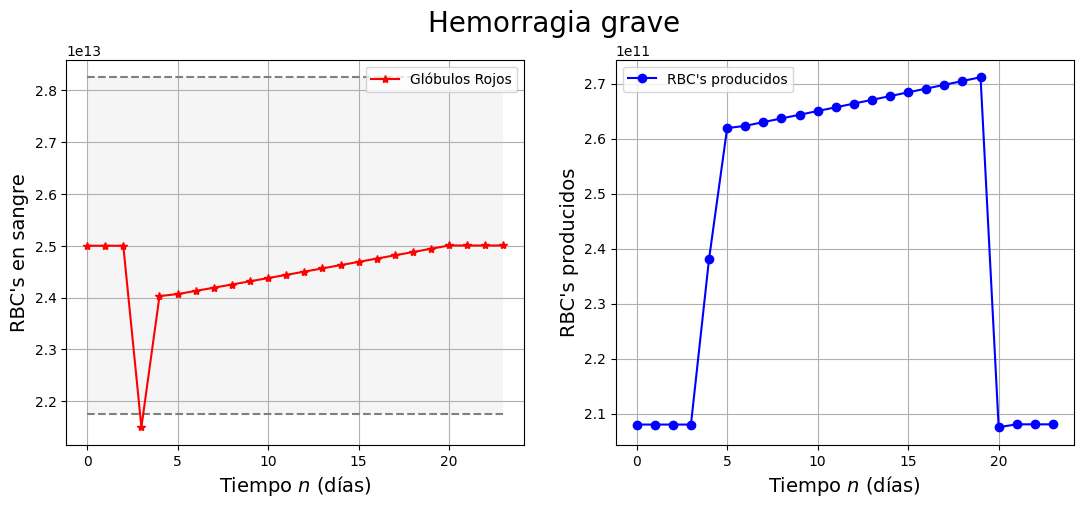
\includegraphics[scale=0.534]{figures/HemoGrave.png}
    \caption{Simulación del modelo para el caso de una hemorragia grave con transfusión. A la izquierda está la gráfica de $R(n)$, a la derecha la de $M(n)$.}
    \label{sec:variaciones:fig:HemoGrave}
\end{figure}

Para los primeros dos días, el cuerpo se encuentra en el estado estable de $\gamma = 1$. En el tercer día ocurre la hemorragia grave y se puede ver una amplia caída en la cantidad de glóbulos en la gráfica izquierda de la figura \ref{sec:variaciones:fig:HemoGrave}. Esta pérdida, sin embargo, se ve mitigada un poco debido a la producción normal de eritrocitos por parte de la médula ósea. A partir de este día inicia el fuerte crecimiento en la producción de RBC's, pues el cuerpo debe intentar recuperar lo perdido (gráfica derecha a partir del cuarto día). En el día cuatro se puede ver el efecto de la transfusión efectuada a través de un gran aumento en la cantidad de eritrocitos respecto al día anterior. En el quinto hay en la gráfica izquierda una disminución en la pendiente respecto al día anterior que se debe a la transición de $\gamma_2$ a $\gamma_3$, y esto se ve reflejado en la primera gráfica por el cambio de pendiente en los días 4-5 y 5-6. A partir del quinto día el cuerpo produce glóbulos rojos según $\gamma_3$ hasta volver al valor inicial y así volver a la estabilidad brindada por $\gamma_1$.

\section{Caso con Anemia Renal}\label{Sec:variaciones:anemia}

Para este caso se considerará un paciente con anemia renal permanente producida por falta de eritropoyetina en el torrente sanguíneo, es decir que los riñones no segregan la suficiente cantidad de la hormona que le indica al cuerpo que debe acelerar la producción de RBC's. Este paciente debe ser tratado por el resto de su vida mediante la aplicación de eritropoyetina por vía intravenosa para poder elevar la producción de eritrocitos por parte de la médula ósea. 

Siguiendo el análisis hecho en la sección \ref{sec:modelo:presentacion}, el parámetro $\gamma$ determina la cantidad de glóbulos rojos producidos por la médula ósea por cada uno eliminado por el bazo. De esta manera, $\gamma$ y la concentración de EPO en el la sangre del paciente están estrechamente relacionados. A continuación se considerará que este parámetro depende de la concentración de eritropoyetina en sangre.

Note que, al hacer esta consideración, entonces se puede adecuar la ecuación $M(n+1)$ de la siguiente manera:

\begin{equation*}
    M(n+1)=\gamma(n)\cdot f \cdot R(n),
\end{equation*}

es decir que la cantidad de glóbulos rojos producidos por la médula ósea en el día $n+1$ ahora también dependerá de la cantidad de glóbulos rojos producidos por cada uno perdido dependiente de EPO en el día $n$, $\gamma(n)$. Esto implica que se debe definir una ecuación para $\gamma(n)$. Esta se basa en el artículo de Frymoyer (\cite{FRYMOYER2019123}), en donde se puede modelar la concentración de una dosis de un fármaco aplicado por vía intravenosa ($\delta(t)$) mediante la ecuación diferencial

\begin{equation}\label{eq:diferencial}
    \dfrac{d\delta}{dt}=-k_e \delta(t),
\end{equation}

en donde $k_e$ es una constante que representa la velocidad a la que el cuerpo elimina el fármaco y es medida en 1/h. Para el caso de la eritropoyetina, Garzone en \cite{GARZONE2012547}, define $k_e=0.077$. La fracción $\dfrac{d\delta}{dt}$ está medida en [(mU/ml)/h], miliunidades por mililitro por hora.

La solución de la ecuación diferencial \ref{eq:diferencial} es:

\begin{equation}\label{eq:solucionDif}
    \delta(t)=\delta_0\cdot e^{-k_e\cdot t},
\end{equation}

donde $\delta_0$ es la concentración de cada dosis.

Para poder modelar múltiples dosis de un fármaco, entonces se debe modificar la solución de la ecuación diferencial para que cuando se deba administrar la nueva dosis (aplicada cada $t_0$ horas), se considere la concentración de fármaco que queda en el cuerpo de la dosis anterior, esto se puede hacer de la siguiente manera:

considere $\delta_n$ como la concentración del fármaco en la sangre en la $n$-ésima dosis, entonce se tiene que 

\begin{align*}
    \delta_0 &= \delta_0,\\
    \delta_1 &= \delta_0 + \delta_0\cdot e^{-k_e\cdot t_0}, \\
    \delta_2 &= \delta_0 + \delta_1\cdot e^{-k_e\cdot t_0}= \delta_0\left(1+e^{-k_e\cdot t_0}+\left(e^{-k_e\cdot t_0}\right)^2\right), \\
    &\cdots \\
    \delta_n &= \delta_0(1+\alpha+\alpha^2+...+\alpha^{n}) \\
    \implies \delta_n &= \delta_0\left(\frac{1-\alpha^{n+1}}{1-\alpha}\right),\quad \alpha=e^{-k_e\cdot t_0}.
\end{align*}

Adecuando este resultado a la ecuación continua \ref{eq:solucionDif} se obtiene que, para cada intervalo entre dos dosis:

\begin{equation*}
    \delta(t) = \delta_{0} \left(\dfrac{1-\alpha^{n}}{1 - \alpha}\right) e^{-(t- (n-1) t_{0})\cdot k_e},
\end{equation*}  

en donde $\alpha = e^{-t_0\cdot k_e}$.

De esta manera, el modelo para un paciente con anemia renal es:
\begin{align}
    R(n+1) &=(1-f)R(n)+M(n), \\
    M(n+1) &=\gamma(n) \cdot f\cdot R(n), \nonumber \\
    \gamma(n+1) &=\dfrac{\epsilon + \delta(24\cdot n)}{\epsilon_s}, \nonumber \\
    \delta(t) = \delta_{0} \left(\dfrac{1-\alpha^{n}}{1 - \alpha}\right) e^{-(t- (n-1) t_{0})\cdot k_e} &; \quad (n-1)t_{0} \leq t < n t_{0}, \quad n=1,2,\dots\nonumber
\end{align}

En donde:
\begin{itemize}
    \item $\epsilon$ es la concentración de EPO en el paciente sin fármaco [mU/ml];
    \item $\epsilon_s$ es la concentración normal de EPO [mU/ml];
    \item $f=0.00832;$ (fracción de RBC's eliminada cada día)
    \item $R(0) = 25\times 10^{12};$ (valor inicial de RBC's)
    \item $M(0) = R(0)\cdot f \cdot 0.809 = 145.6\times 10^{9};$ (RBC's eliminados por la médula ósea en el día 0)
    \item $\delta_0$ es la concentración de cada dosis [mU/ml];
    \item $k_e=0.077.$ (constante de eliminación) [$\textrm{h}^{-1}$];
    \item $t_0$ es el tiempo que debe pasar entra cada dosis [h].
\end{itemize}

El valor $24\cdot n$ en la función $\delta(t)$ para calcular $\gamma(n)$ se utiliza para acoplar el modelo continuo de la concentración del fármaco al modelo base, que es discreto. El valor $24 \cdot n$ indica la concentración del fármaco al comienzo del día $n$, pues $t$ se mide en horas.

Para poder definir los parámetros de las ecuaciones, se seguirá el estudio de Panjeta (\cite{panjeta2017interpretation}) sobre la concentración de EPO en pacientes con anemia renal. Para el grupo de pacientes sin anemia, el promedio de EPO en sangre fue de 11.0 mU/ml, mientras que para el grupo con anemia renal de etapa 4 fue de 8.9 mU/ml. Dado que el valor de $\gamma(n)$ está dado en una fracción, entonces se tomará que el valor normal $\epsilon =$ 11.0 mU/ml de EPO. Para los pacientes con anemia renal de cuarta etapa, se tendría que $\epsilon = 8.9$ mU/ml.

El siguiente paso para las simulaciones es establecer la concentración de dosis que se le debe inyectar al paciente.

\subsection{Concentración de Dosis  = 0.975 mU/ml}

Como se expuso en la sección \ref{subsec:RBC:enfermedades:anemia}, el tratamiento de inyección de EPO depende de la masa corporal del paciente, se debe encontrar una masa corporal en el que basar la dosis pra el modelo. Siguiendo el estudio realizado por el periódico el Tiempo en \cite{elTiempo}, la altura promedio de un hombre colombiano en 2021 es de aproximadamente 172 cm. Utilizando el índice de masa corporal (\cite{IMC}), una medida para hallar el rango de masa corporal ideal según la estatura de una persona, la masa corporal ideal de un hombre que mide 172 cm de altura es de aproximadamente unos 65 kg. De esta manera, la dosis de EPO que se tendrá en cuenta para la primera simulación de esta variación del modelo es de 4875 unidades cada tres días (0.975 mU/ml).

Así, para la concentración de 0.975 mU/ml de EPO, se tienen los siguientes valores:

\begin{itemize}
    \item $\epsilon = 8.9$ es la concentración de EPO en el paciente sin fármaco [mU/ml];
    \item $\epsilon_s = 11$ es la concentración normal de EPO [mU/ml];
    \item $f=0.00832;$ (fracción de RBC's eliminada cada día)
    \item $R(0) = 25\times 10^{12};$ (valor inicial de RBC's)
    \item $M(0) = R(0)\cdot f \cdot 0.809 = 145.6\times 10^{9};$ (RBC's eliminados por la médula ósea en el día 0)
    \item $\delta_0=0.975$ es la concentración de cada dosis [mU/ml];
    \item $k_e=0.077.$ (constante de eliminación) [$\textrm{h}^{-1}$];
    \item $t_0=72$ es el tiempo que debe pasar entra cada dosis [h].
\end{itemize}

Como bien se puede ver en la figura \ref{sec:variaciones:fig:Anemia1}, la dosis de EPO administrada no es suficiente para sanar la constante pérdida de glóbulos rojos en el paciente, pues $R(n)$ presenta una disminución en el tiempo, que al infinito se vuelve 0. Esto ocurre dado que $\gamma + \delta_0=9.875 < \gamma_s$, y ya que la concentración del fármaco se estabiliza rápido, nunca se llega a la concentración esperada de 11 mU/ml para lograr la estabilización. Sin embargo, la simulación muestra como cada dosis aplicada hace que el cuerpo aumente de una manera significativa su producción de eritrocitos, como se ve en la gráfica para $M(n)$.

\begin{figure}[H]
    \centering
    \captionsetup{justification=centering}
    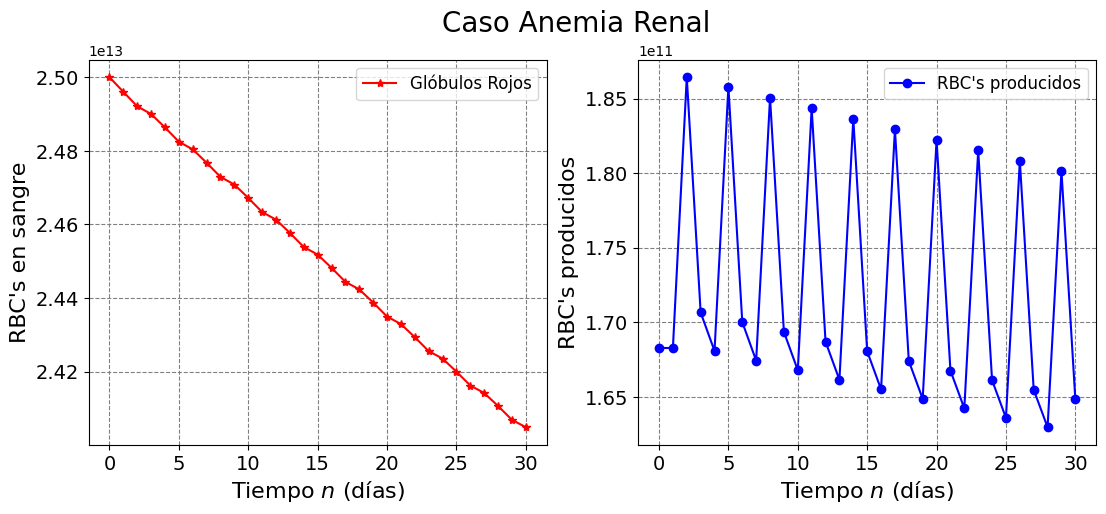
\includegraphics[scale=0.534]{figures/AR11.png}
    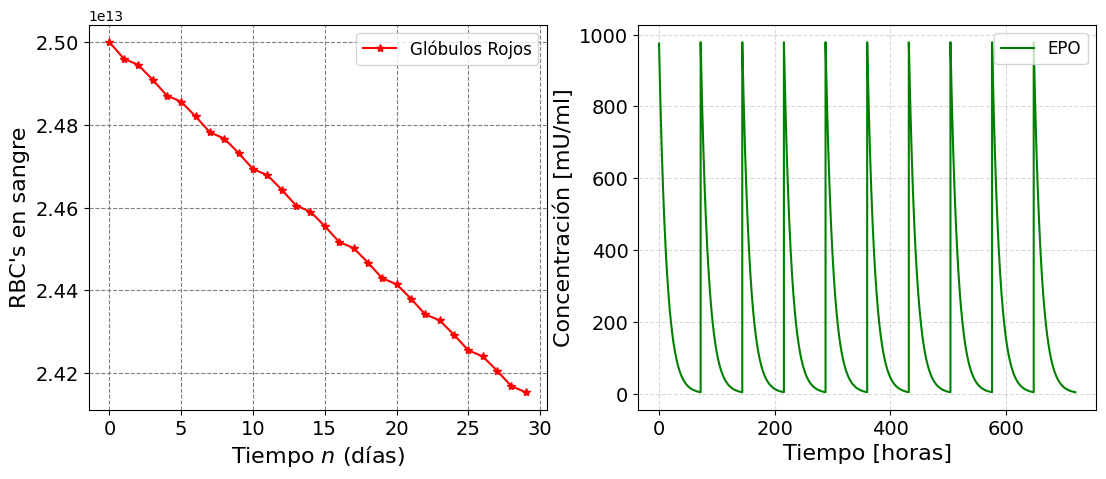
\includegraphics[scale=0.8]{figures/AR12.png}
    \caption{Simulación del modelo para el caso de anemia renal con dosis de EPO de 0.975 mU/ml. A la izquierda está la gráfica de $R(n)$, a la derecha la de $M(n)$, abajo la de $\delta(t)$.}
    \label{sec:variaciones:fig:Anemia1}
\end{figure}

Se concluye que la dosis aplicada de 0.975 mU/ml no es suficiente para que se contrarresten los efectos de la anemia renal del paciente. De esta manera, se debe encontrar un valor de la dosis para que el paciente logre estabilizar su cantidad de eritrocitos.

\subsection{Concentración de Dosis = 5.307 mU/ml}

Para hallar una concentración de dosis que permita lograr los resultados esperados, se realizaron varias simulaciones para hallar una concentración de la dosis que permita una estabilidad en la cantidad de glóbulos rojos del paciente. Con una dosis de $\delta_0 = 5.307$ [mU/ml] se logra llegar a la estabilidad esperada.

Para la concentración de 5.307 mU/ml de EPO, se tienen los siguientes valores:

\begin{itemize}
    \item $\epsilon = 8.9$ es la concentración de EPO en el paciente sin fármaco [mU/ml];
    \item $\epsilon_s = 11$ es la concentración normal de EPO [mU/ml];
    \item $f=0.00832;$ (fracción de RBC's eliminada cada día)
    \item $R(0) = 25\times 10^{12};$ (valor inicial de RBC's)
    \item $M(0) = R(0)\cdot f \cdot 0.809 = 145.6\times 10^{9};$ (RBC's eliminados por la médula ósea en el día 0)
    \item $\delta_0=5.307$ es la concentración de cada dosis [mU/ml];
    \item $k_e=0.077.$ (constante de eliminación) [$\textrm{h}^{-1}$];
    \item $t_0=72$ es el tiempo que debe pasar entra cada dosis [h].
\end{itemize}

La figura \ref{sec:variaciones:fig:Anemia2} muestra como, gracias a la nueva dosis, el cuerpo es capaz de lograr una oscilación constante para un valor máximo de RBC's ligeramente menor al original. La función $R(n)$ se vuelve periódica con un máximo de $24.9817$ glóbulos rojos, menos del $1\%$ de pérdida respecto al valor original.

\begin{figure}[H]
    \centering
    \captionsetup{justification=centering}
    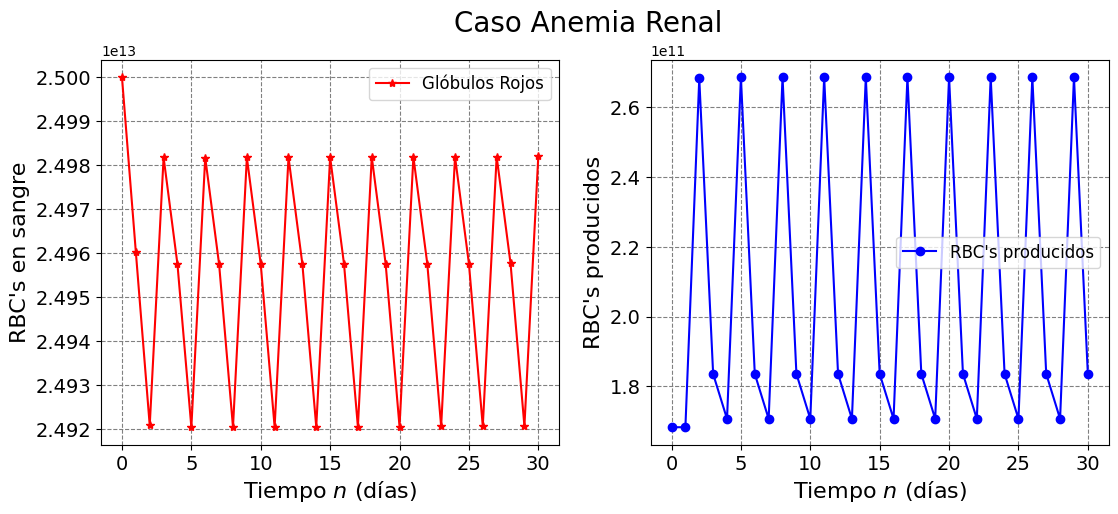
\includegraphics[scale=0.526]{figures/AR21.png}
    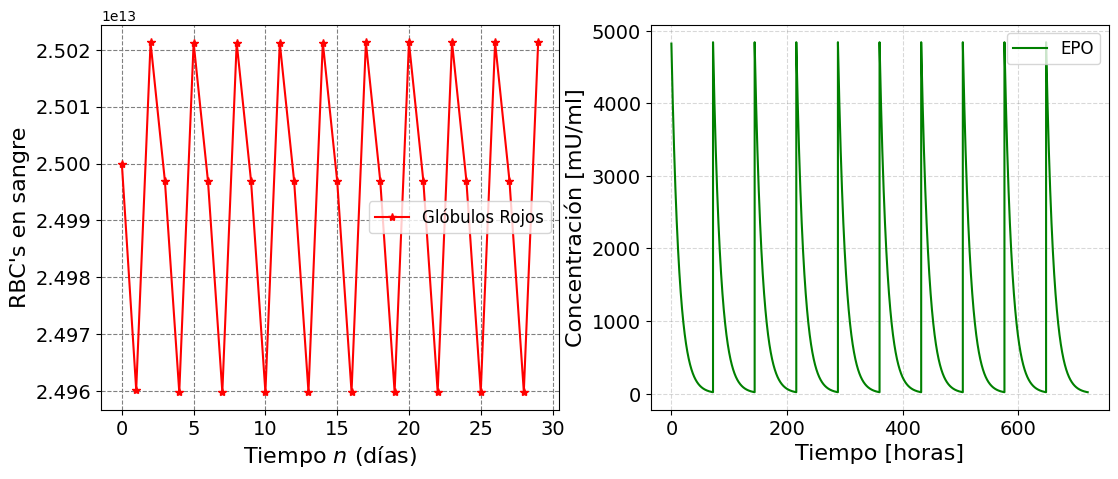
\includegraphics[scale=0.8]{figures/AR22.png}
    \caption{Simulación del modelo para el caso de anemia renal con dosis de EPO de 5.309mU/ml. A la izquierda está la gráfica de $R(n)$, a la derecha la de $M(n)$, abajo la de $\delta(t)$.}
    \label{sec:variaciones:fig:Anemia2}
\end{figure}


\chapter{Conclusiones y trabajo a futuro}\label{chap:Conclusiones}

Habiendo hecho ya los análisis, simulaciones y variaciones del modelo base, es hora de evidenciar los hallazgos principales de la investigación, las limitaciones que presenta el modelo y la importancia de la investigación para trabajos futuros.

\section{Resumen de los hallazgos principales}

Las variaciones del modelo, presentadas en las ecuaciones \ref{eq:HemoLeveMal}, \ref{eq:HemoLeveBien}, \ref{eq:HemoGrave} y \ref{eq:ModeloAnemia} fueron producto de un análisis meticuloso de las simulaciones y de el estudio fisiológico de las dinámicas de los glóbulos rojos presentado en el capítulo \ref{chap:RBC}. 

Para el caso de la hemorragia leve (sección \ref{subsec:variaciones:hemorragia:leve}), el cambio entre las ecuaciones \ref{eq:HemoLeveMal} y \ref{eq:HemoLeveBien} es fundamental ya que logra que los resultados obtenidos sean los esperados, pues la producción de RBC's debe aumentar si hay alguna pérdida ya que el cuerpo es el encargado de mantener su homeostasis. Es verdad que la pérdida presentada no es muy grave respecto a la concentración normal y que el paciente podría vivir sin esta cantidad de eritrocitos, pero se debe asumir que el cuerpo recupera sus eritrocitos de manera natural, garantizando la homeostasis.

El análisis para las hemorragias leves fue clave para poder plantear el modelo de hemorragias graves \ref{eq:HemoGrave} en la sección \ref{subsec:variaciones:hemorragia:grave}, pues al evidenciar que el cuerpo debe de aumentar su producción de RBC's después de la pérdida es que se pueden plantear los diferentes casos para $M(n)$. El análisis fisiológico hecho para este caso también permitió que después de la transfusión se cambiara de $\gamma_2$ a $\gamma_3$ para evitar una recuperación muy lenta del paciente.

Es muy interesante notar como un ligero cambio en los parámetros del modelo \ref{eq:ModeloAnemia} presenta resultados tan diferentes para la gráfica de $R(n)$, pues en la sección \ref{subsec:variaciones:anemia:mal} hay una disminución casi lineal de eritrocitos en la figura \ref{sec:variaciones:fig:Anemia1} mientras que en la sección \ref{subsec:variaciones:anemia:bien} se logra una oscilación de los valores de RBC's cada tres días según la figura \ref{sec:variaciones:fig:Anemia2}. Este cambio en la dosis lo es todo, y es fundamental para que un paciente pueda llevar una vida plena a pesar de su enfermedad, pues la cantidad de glóbulos rojos que presenta el paciente tanto en los picos como en los valles de la gráfica no representa una pérdida significativa de eritrocitos. Se debe recalcar que la concentración de la dosis depende de su grado de anemia; al aumentar la dosis aumenta la producción de glóbulos rojos y en ningún caso se quiere llegar a una sobrepoblación de células en el torrente sanguíneo. Es de vital importancia determinar el nivel medio de EPO en la sangre del paciente antes de tratar la anemia renal.

\section{Limitaciones del modelo}

Los modelos matemáticos brindan aproximaciones para intentar comprender un problema. Para el caso presente el problema es médico, y al ser el cuerpo humano un sistema en el que cada uno de sus componentes tiene relevancia en los demás, entonces las aproximaciones que brindan los modelos matemáticos tienen sus limitaciones. Todos los modelos planteados a lo largo de la investigación no son la excepción de esta regla y se podrían mejorar al tener en cuenta otras variables.

Uno de los componentes principales de los eritrocitos es la hemoglobina, compuesta principalmente por hierro. Así, los niveles de hierro en el cuerpo son un factor que se podría tener en cuenta a la hora de plantear un nuevo modelo. Sin suficiente cantidad de hierro en el cuerpo, no hay hemoglobina, y sin hemoglobina los glóbulos rojos pierden su función.

Teniendo esto en cuenta, también sería interesante incluir al modelo cierta información del paciente: su masa corporal, su edad, sus hábitos alimenticios, su ubicación geográfica o su sexo. Esta información es muy importante ya que el cuerpo humano funciona de un modo diferente para cada persona. De esta manera, otra limitación importante del modelo se encuentra en sus parámetros y valores iniciales. Al desestimar cierta información del paciente se pierden datos importantes para calibrar estos valores: la cantidad inicial de RBC's, por ejemplo, se tomó para el caso promedio de hombres adultos en perfecta condición física, los valores de $\gamma$ utilizados en la sección \ref{sec:modelo:simulaciones}, por poner otro ejemplo, fueron escogidos arbitrariamente y no reflejan ninguna condición específica del paciente. 

Sería interesante considerar que los valores de EPO en sangre no son constantes para una persona, pues dependen de los niveles de oxígeno. Así, los niveles de eritropoyetina en sangre van cambiando según lo necesite el cuerpo. De esta manera, se podría agregar al modelo base, así como se hace para el caso de la anemia renal, una función para determinar los valores de $\gamma$ en el tiempo.

Finalmente, y en especial para el caso de la anemia renal, los resultados podrían mejorar si se considera un modelo continuo en vez de uno discreto. El cuerpo consume a gran velocidad la EPO administrada (véanse las figuras \ref{sec:variaciones:fig:Anemia1} y \ref{sec:variaciones:fig:Anemia2} para la gráfica de la concentración de EPO), y al tomar un modelo que mide día a día la concentración de EPO se pierde una buena cantidad de droga administrada. Para el caso de las hemorragias, un cambio a un modelo continuo sería beneficioso, pues el sangrado debe de ser tratado con la mayor velocidad posible, no de un día para otro; además, la transfusión sanguínea es un proceso que toma cierto tiempo y no es inmediato. 

\section{Posibles direcciones para investigaciones futuras}

En la sección \ref{Sec:variaciones:anemia} se propuso un modelo para reflejar la aplicación de EPO en la sangre del paciente. Esta variación se podría mejorar si se conoce bien el proceso de la síntesis de eritropoyetina por parte del cuerpo y cómo esta afecta la producción de glóbulos rojos.

Una de las interesantes direcciones futuras que se podría tomar para el proyecto es utilizar herramientas tecnológicas que permitan mejorar los valores de los parámetros y resolver ciertas limitaciones previamente mencionadas. Se propone utilizar inteligencia artificial y análisis estadísticos de bases de datos de hospitales, ya que pueden brindar información muy útil que permita ser más acertados en la construcción del modelo como la inclusión de nuevas variables para que los modelos puedan servir para cada paciente en particular en vez de en un caso general.

Como se ha visto a lo largo del proyecto, las células madre tienen un rol fundamental a la hora de la producción de glóbulos rojos. Su función no se limita únicamente a los eritrocitos: las células madre son las encargadas de la generación de casi todas las células especializadas del cuerpo humano. Una de las principales investigaciones actuales en la medicina se basa en la \textbf{movilización de células madre}, que es el proceso mediante el cual se provoca médicamente la migración de células madre a la sangre para posteriormente extraerlas y conservarlas para un posible trasplante de células madre. Un trasplante de células madre es útil para los pacientes con ciertos tipos de cáncer como la leucemia, pues al eliminar células cancerosas del cuerpo, las nuevas células madre obtenidas con el trasplante se encargarán de reemplazar las células eliminadas con células sanas (\cite{Trasplante}).  

Conocer las dinámicas de los glóbulos rojos (y, en general, de la sangre) matemáticamente es muy útil desde un punto de vista médico, pues para la movilización de células madre se puede sacar ventaja de los análisis matemáticos para poder lograr un mejor procedimiento, que pueda salvar o mejorar la vida de un paciente con cáncer.


\nocite{*}

\printbibliography
\appendix

\chapter{Example Appendix}

Here you might present some additional results, derivations, proofs etc. that were not included in the main text.

\section{Useful Bounds}

We include some bounds that are useful in the proofs of the main results.

\begin{proposition}\label{ap:prop:upperbinom}
    $\binom{n}{k} \leq \left(\frac{en}{k}\right)^k$ for $1 \leq k \leq n$. 
\end{proposition}

\begin{proposition}\label{ap:prop:lowebinom}
    $\left(\frac{n}{k}\right)^k \leq \binom{n}{k}$ for $1 \leq k \leq n$.
\end{proposition}

\begin{proposition}\label{ap:prop:exp}
    $(1 - p) \leq e^{-p}$ for $0 \leq p \leq 1$.
\end{proposition}

\textbf{Proof. } The Taylor series of $e^{-p}$ is decreasing and alternating, so
\[e^{-p} = 1 - p + \frac{p^2}{2!} - \frac{p^3}{3!} + ... \geq 1 - p.\]

\begin{proposition}
    $\binom{n}{k}^2 \leq \binom{2n}{2k}$ for $n \geq 1$. 
\end{proposition}

\textbf{Proof. } We have that

% Optional; if you've written code, you want to include some basic
% documentation. Also include the git repository details if you have
% published the code.

% \chapter{Software Documentation}

% This is totally free-form - you can break it down by chapter, or integrate
% it. This is not at all critical.

% Set this up for MATLAB - you can tweak it for other languages. This could go in the toplevel preamble if you prefer.

\lstset{
	tabsize=4,
	rulecolor=,
	language=Matlab,
	basicstyle=\tiny,
	upquote=true,
	aboveskip={1.5\baselineskip},
	columns=fixed,
	showstringspaces=false,
	extendedchars=true,
	breaklines=true,
	prebreak = \raisebox{0ex}[0ex][0ex]{\ensuremath{\hookleftarrow}},
	frame=single,
	showtabs=false,
	showspaces=false,
	showstringspaces=false,
	identifierstyle=\ttfamily,
	keywordstyle=\color[rgb]{0,0,1},
	commentstyle=\color[rgb]{0.133,0.545,0.133},
	stringstyle=\color[rgb]{0.627,0.126,0.941},
	numbers=left, numberstyle=\tiny, stepnumber=1,
	numbersep=5pt
}

Here's an example source code listing, where the code is read in from an external file:

\lstinputlisting{code/animation.m}

\section{Code Availability}
All scripts and source code used for simulation and analysis of the ... are available here
 % example
 \lstinputlisting{code/animation.m}
\url{https://bitbucket.org/username/gitrepo.git}

\section{Software Requirements}
\begin{itemize}
\item MATLAB code is confirmed working with version XXXX;
\item Simulations require the use of gcc version XXX or llvm/clang version YYYY
\end{itemize}

\section{Simulation Code - How to Run}

% Some examples of using the code - sample workflow


\end{document}
